\documentclass[a4paper,12pt]{report}
\usepackage[left=2cm,right=2cm,top=2cm,bottom=3cm]{geometry}
\usepackage[utf8]{inputenc}
\usepackage[T1]{fontenc}
\usepackage{libertine}
\usepackage[scaled]{beramono}
%\usepackage{fontawesome}
\usepackage{fontawesome5}
\usepackage[portuges]{babel}
\usepackage{hyperref}
\usepackage{graphicx}
\graphicspath{{Figuras/}}
\DeclareGraphicsExtensions{.pdf,.png}
\usepackage{xspace}
\usepackage{booktabs}
\usepackage{multirow}
% \usepackage{amsmath}
% \usepackage{amsfonts}
% \usepackage{amssymb}
\usepackage{listings}
\usepackage{xcolor}
%\usepackage{caption} \captionsetup[table]{skip=3pt}
\usepackage{setspace}
\usepackage{enumitem}
\usepackage[brazilian,nameinlink]{cleveref}
%\singlespacing
\onehalfspacing
%\doublespacing
%\setstretch{1.1}

\usepackage{titlesec}
%\titlelabel{\thetitle.\quad}
\titlespacing\section{0pt}{12pt plus 4pt minus 2pt}{0pt plus 2pt minus 2pt}
\titlespacing\subsection{0pt}{12pt plus 4pt minus 2pt}{0pt plus 2pt minus 2pt}
\titlespacing\subsubsection{0pt}{12pt plus 4pt minus 2pt}{0pt plus 2pt minus 2pt}

\usepackage[os=win]{menukeys}\renewmenumacro{\keys}[+]{shadowedroundedkeys}
\usepackage[lang={english},type={CC},modifier={by},version={4.0}]{doclicense}

%Cabeçalho e rodapé
\usepackage{fancyhdr}
\setlength{\headheight}{52pt}
\fancypagestyle{plain}{% Definição das páginas de capítulo
  \fancyhf{}%
  \fancyfoot[r]{\thepage}%
  \renewcommand{\headrulewidth}{0pt}% Line at the header invisible
  \renewcommand{\footrulewidth}{0pt}% Line at the footer visible
}

\pagestyle{fancy}
\fancyhf{}
\lhead{\slshape\nouppercase{\leftmark}}
\fancyfoot[R]{\thepage}

\widowpenalty100000
\clubpenalty100000

\title{Laboratório de Redes de Computadores \\ com Cisco Packet Tracer}
\author{Prof. André Leon S. Gradvohl, Dr.\\\href{mailto://gradvohl@ft.unicamp.br}{gradvohl@ft.unicamp.br}}
\date{18 de janeiro de 2023}

\hypersetup{
    pdfstartview={XYZ null null .75}, %Abre a página em 100%
    pdfcreator=pdflatex,
    pdfdisplaydoctitle=true,
    pdftitle={Laboratório de Redes de Computadores com Cisco Packet Tracer},
    pdfauthor={André Leon Gradvohl Dr},
    pdfsubject={Tutorial para a prática de Redes de Computadores com o software Cisco Packet Tracer},
    pdfkeywords={Redes de Computadores -- Cisco Packet Tracer -- Práticas}
}

\newcommand{\Comando}[1]{{\color{blue}\texttt{#1}}}
%
\newcommand{\ComandoParametros}[2]{%
\mbox{\textcolor{blue}{\texttt{#1}}%
\xspace\textcolor{red}{\texttt{#2}}}%
}%fim ComandoParametros

\newcommand{\ComandoDoisParametros}[3]{%
\textcolor{blue}{\texttt{\textbackslash{#1}}}%
\textcolor{red}{\texttt{\{}}%
\texttt{#2}%
\textcolor{red}{\texttt{\}}}%
\textcolor{red}{\texttt{\{}}%
\texttt{#3}%
\textcolor{red}{\texttt{\}}}%
}%fim ComandoDoisParametros

\definecolor{codegreen}{rgb}{0,0.6,0}
\definecolor{codegray}{rgb}{0.5,0.5,0.5}
\definecolor{codepurple}{rgb}{0.58,0,0.82}
\definecolor{backcolour}{rgb}{0.95,0.95,0.92}
\definecolor{orcidlogocol}{HTML}{A6CE39}
\definecolor{twitterlogocol}{RGB}{29,161,242}
\definecolor{linkedinlogocol}{RGB}{10,102,194}
\definecolor{mastodonlogocol}{RGB}{160,32,240}

\lstdefinestyle{MyCStyle}{language=C,
  belowcaptionskip=1\baselineskip,
  breaklines=true,
  postbreak=\mbox{\textcolor{blue}{$\hookrightarrow$}\space},
  xleftmargin=\parindent,
  showstringspaces=false,
  basicstyle=\linespread{.8}\footnotesize\fontencoding{T1}\fontfamily{fvm}\selectfont,
   %identifierstyle=\color{blue},
  commentstyle=\color{codegreen},
  keywordstyle=\color{magenta},
  numberstyle=\tiny\color{codegray},
  stringstyle=\color{codepurple},
  frame = single, 
}

\newcommand{\lstprompt}{\$}
\renewcommand*\thelstnumber{\lstprompt}
\lstdefinestyle{MyBashStyle}{language=bash,
  basicstyle=\fontencoding{T1}\fontfamily{fvm}\selectfont,
  %xleftmargin=\parindent,
  xleftmargin=2.7ex,
  morecomment=[s][\color{red}]{-}{\ }, 
  morecomment=[s][\color{red}]{--}{\ },
  morekeywords={uname,gcc,top,grep,ping,ip,bandwidth},%
  showstringspaces=false,
  commentstyle=\color{orange},
  keywordstyle=\color{blue},
  numbers=left,
  numberstyle=\color{codegreen}\fontencoding{T1}\fontfamily{fvm}\selectfont\,
}

\lstdefinestyle{outputStyle}{
    basicstyle=\footnotesize\fontencoding{T1}\fontfamily{fvm}\selectfont,
    identifierstyle=\color{black},
    breakatwhitespace=false,         
    breaklines=true,                 
    captionpos=b,                    
    keepspaces=true,                 
    showspaces=false,                
    showstringspaces=false,
    showtabs=false,                  
    xleftmargin=\parindent,
    postbreak=\mbox{\textcolor{blue}{$\hookrightarrow$}\space},
}

\newcommand{\CPT}{Cisco Packet Tracer\xspace}
\newcommand{\semaspas}[1]{\enquote{\texttt{#1}} {\footnotesize (sem aspas)}\xspace}

\begin{document}

\maketitle

\tableofcontents

\setlength\parindent{0pt} %Sem identação no documento
\setlength{\parskip}{1em} %espaço entre parágrafos


\chapter{Introdução}\label{chp:introducao}
O objetivo deste texto é propor algumas atividades práticas para a consolidação dos conceitos abordados na disciplina Redes de Comunicação I. Essa disciplina é oferecida na Faculdade de Tecnologia da Universidade Estadual de Campinas (FT/UNICAMP) para os cursos Bacharelado em Sistemas de Informação e Tecnologia em Análise e Desenvolvimento de Sistemas.

Esse material pode ser utilizado por qualquer pessoa, de qualquer curso ou instituição, desde que respeitadas as condições da licença CC-BY-4.0, descrita na \Cpageref{chp:licenca}. Informações de como obter o material também estão nessa página.

Supõe-se que o estudante leitor deste material já tenha instalado o \CPT. Caso ainda não tenha instalado, o estudante poderá fazê-lo a partir dos passos a seguir:

\begin{enumerate}[label*=\arabic*.]
    \item Acesse o site \url{https://www.netacad.com/courses/packet-tracer}
    \item Agora, você deve cadastrar-se no site.
    \begin{enumerate}[label*=\arabic*.]
        \item No canto superior direito, clique na opção \enquote{\textit{login}}.
        \item Na parte inferior da nova página, Registre-se.
    \end{enumerate}
    \item Depois de cadastrado e já na sua área, clique na opção \enquote{Recursos} e, em seguida, \enquote{Baixar o Packet Tracer}.
    \item No final da nova página carregada, escolha a versão mais adequada para o sistema operacional que você vai utilizar.
\end{enumerate}

Se a instalação aconteceu corretamente, execute o \CPT. A tela inicial do software deve ser parecida com aquela ilustrada na \Cref{fig:telaInicial}. Note que há duas visões possíveis para a rede que vamos montar ou simular: a visão lógica (\textit{Logical}) e a visão física (\textit{Physical}). Nós vamos nos concentrar na visão lógica.

\begin{figure}[!htb]
    \centering
    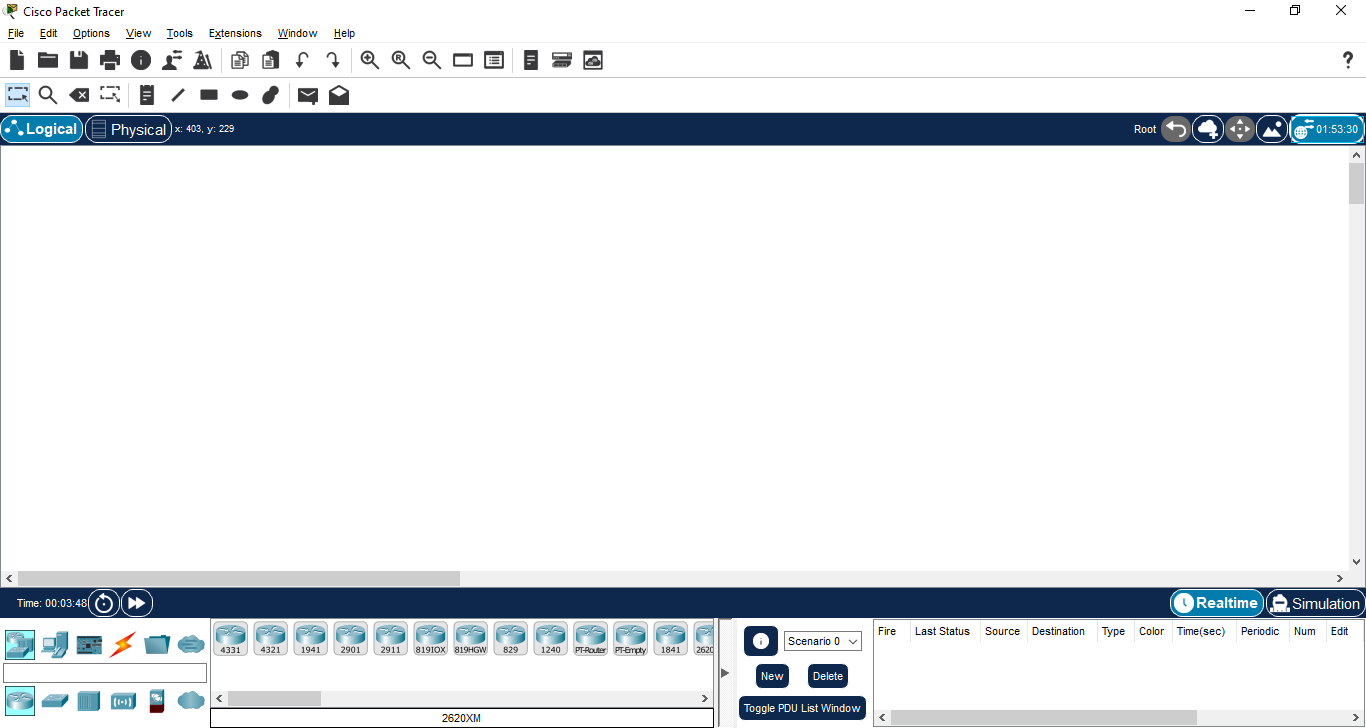
\includegraphics[width=.99\textwidth]{Figuras/TelaInicial}
    \caption{Tela inicial do \CPT.}    \label{fig:telaInicial}
\end{figure}

Ainda na tela da \Cref{fig:telaInicial}, na parte de baixo, à esquerda, note que temos vários elementos para as redes de comunicação. Esses elementos vão desde dispositivos internos da rede (\textit{Network Devices}) até dispositivos finais (\textit{End Devices}), incluindo os elementos para as conexões (cabeamento). Utilizaremos esses elementos nos exercícios ao longo deste tutorial.

\section{Exercício}
Como exercício, familiarize-se com os elementos que compõem uma rede de computadores. Usando o \CPT, tente identificar os seguintes elementos:
\begin{itemize}
    \item Roteadores, \textit{switches} e \textit{hubs}.
    \item PCs, \textit{notebooks} e servidores.
    \item Dispositivos para internet das coisas (por exemplo, um detector de monóxido de carbono \textit{online}).
    \item Cabo coaxial, cabo de cobre (par trançado), cabo de cobre \textit{cross-over}, fibra óptica.
\end{itemize}

\chapter{Criação de redes simples -- \textit{Cross-over}, \textit{hub} e \textit{switch}}\label{chp:redesSimples}

Neste capítulo, vamos ver como criar uma rede bem simples, de um computador para outro (um \textit{notebook}) de uma forma direta na \Cref{sec:conexDireta}. Depois, vamos criar uma pequena rede local (\textit{Local Area Network} -- LAN) um pouco mais complexa, com mais computadores conectados. 

Para as redes mais complexas vamos usar, primeiro, um \textit{hub}, para implementar a topologia barramento na \Cref{sec:conexHub}. Depois, usando um \textit{switch}, vamos implementar a topologia estrela na \Cref{sec:conexSwitch}. 
Não esqueça de executar o \CPT para realizar os exercícios a seguir.

\section{Conexão direta entre computadores}\label{sec:conexDireta}

Para estabelecer uma conexão direta entre dois computadores, precisamos criar um ambiente com dois desses dispositivos (um PC e um \textit{laptop}) e um cabo \textit{cross-over}. Para tanto, execute os passos a seguir.

\begin{enumerate}[label*=\arabic*.]
    \item Adicione um PC e um \textit{laptop} (\textit{End Devices}) no seu ambiente, arrastando os respectivos ícones para a área em branco.
    \item Dentre as conexões (\textit{Connections}), selecione um cabo \textit{cross-over}; depois, ligue o PC ao \textit{laptop}. 
    \begin{enumerate}[label*=\arabic*.]
       \item Ao estabelecer a conexão, escolha a interface física \enquote{\textit{Fast ethernet}} em ambos os dispositivos.
    \end{enumerate}
\end{enumerate}

A \Cref{fig:conexaoCrossover} mostra como deve ficar a tela no \CPT após a realização desse primeiro passo. Note que os triângulos verdes próximos a cada dispositivo indicam que eles estão conectados.

\begin{figure}
    \centering
    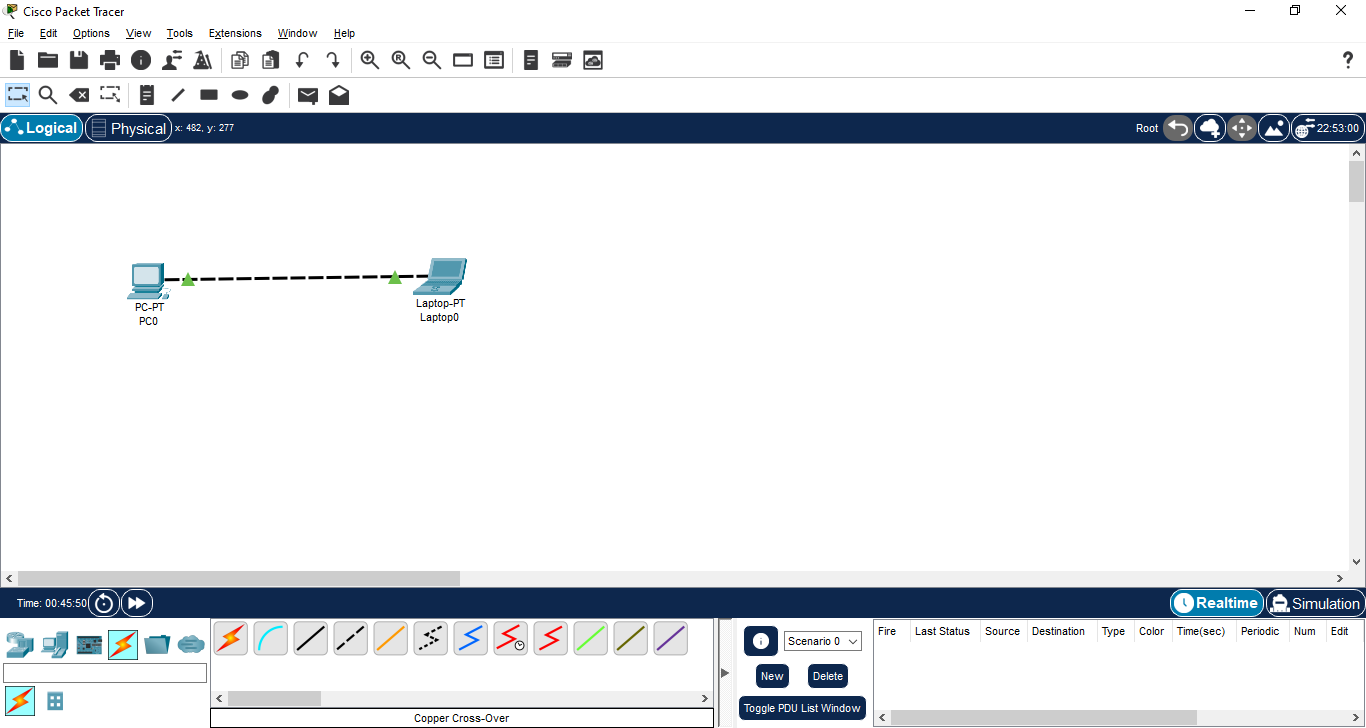
\includegraphics[width=.99\textwidth]{Figuras/ConexaoCrossover}
    \caption{Conexão direta com cabo \textit{cross-over}.}\label{fig:conexaoCrossover}
\end{figure}

Vamos agora realizar uma configuração estática básica para a conexão desses computadores. Para isso, siga os seguintes passos:

\begin{enumerate}
    \item Clique no dispositivo.
    \item Na parte superior da nova janela aberta, clique na opção \textit{Desktop}.
    \item Selecione o ícone em que está escrito \textit{IP Configuration}.
    \item Na caixa de texto em que está escrito \textit{IPv4 Address}, informe o endereço IP do dispositivo (veja quais são a seguir).
\end{enumerate}

Nesse caso, utilizaremos o IP \texttt{10.0.0.5} para o PC e o IP \texttt{10.0.0.6} para o \textit{laptop}. Perceba que, após a inserção do endereço IP, a máscara \texttt{255.0.0.0} é automaticamente inserida também.

\subsection{Verificação da conexão entre os componentes}\label{subsec:verificaConex}
Vejamos agora se ambos os componentes conseguem trocar dados. Para isso utilizaremos o comando \Comando{ping}. execute os passos a seguir:

\begin{enumerate}
    \item Clique em um dos dispositivos (por exemplo, o PC).
    \item Na parte superior da nova janela aberta, clique na opção \textit{Desktop}.
    \item Selecione o ícone em que está escrito \textit{Command Prompt}.
    \item Execute o comando a seguir e veja o resultado.
    \begin{lstlisting}[style=MyBashStyle]
ping 10.0.0.6
    \end{lstlisting}
\end{enumerate}

\section{Exercício}
Repita o mesmo procedimento anterior, dessa vez para o \textit{laptop}. Não esqueça que, nesse caso, você deve informar para o comando \Comando{ping} o endereço IP do PC (\texttt{10.0.0.5}).

Apenas como ilustração, tente informar um endereço IP de um dispositivo que não existe ainda nessa rede (por exemplo, \texttt{10.0.0.7}).

\section{Conexão de vários computadores com um \textit{hub}}\label{sec:conexHub}
Vamos criar uma pequena rede local com três computadores (PCs), interligados por um \textit{hub}. Essa rede formará uma topologia do tipo barramento. Para tanto, execute os passos a seguir.

\begin{enumerate}[label*=\arabic*.]
    \item Adicione três PCs no seu ambiente, arrastando os respectivos ícones para a área em branco.
    \item Adicione  um \textit{hub} (\textit{Network Device}) no seu ambiente.
    \item Dentre as conexões, selecione um cabo de cobre (par trançado); depois, ligue cada um dos PCs ao \textit{hub}. 
    \begin{enumerate}[label*=\arabic*.]
       \item Ao estabelecer a conexão, escolha a interface física \enquote{\textit{Fast ethernet}} em ambos os dispositivos.
    \end{enumerate}
    \item Configure os endereços IP de cada um dos PCs (\texttt{10.0.0.5}, \texttt{10.0.0.6} e \texttt{10.0.0.7}) e a máscara \texttt{255.0.0.0}.
\end{enumerate}

Feita a configuração, verifique usando o comando \Comando{ping}, se todos os computadores estão acessíveis, um a partir do outro. Para isso, use o procedimento da \Cref{subsec:verificaConex}. A \Cref{fig:hub} ilustra a topologia criada.

\begin{figure}
    \centering
    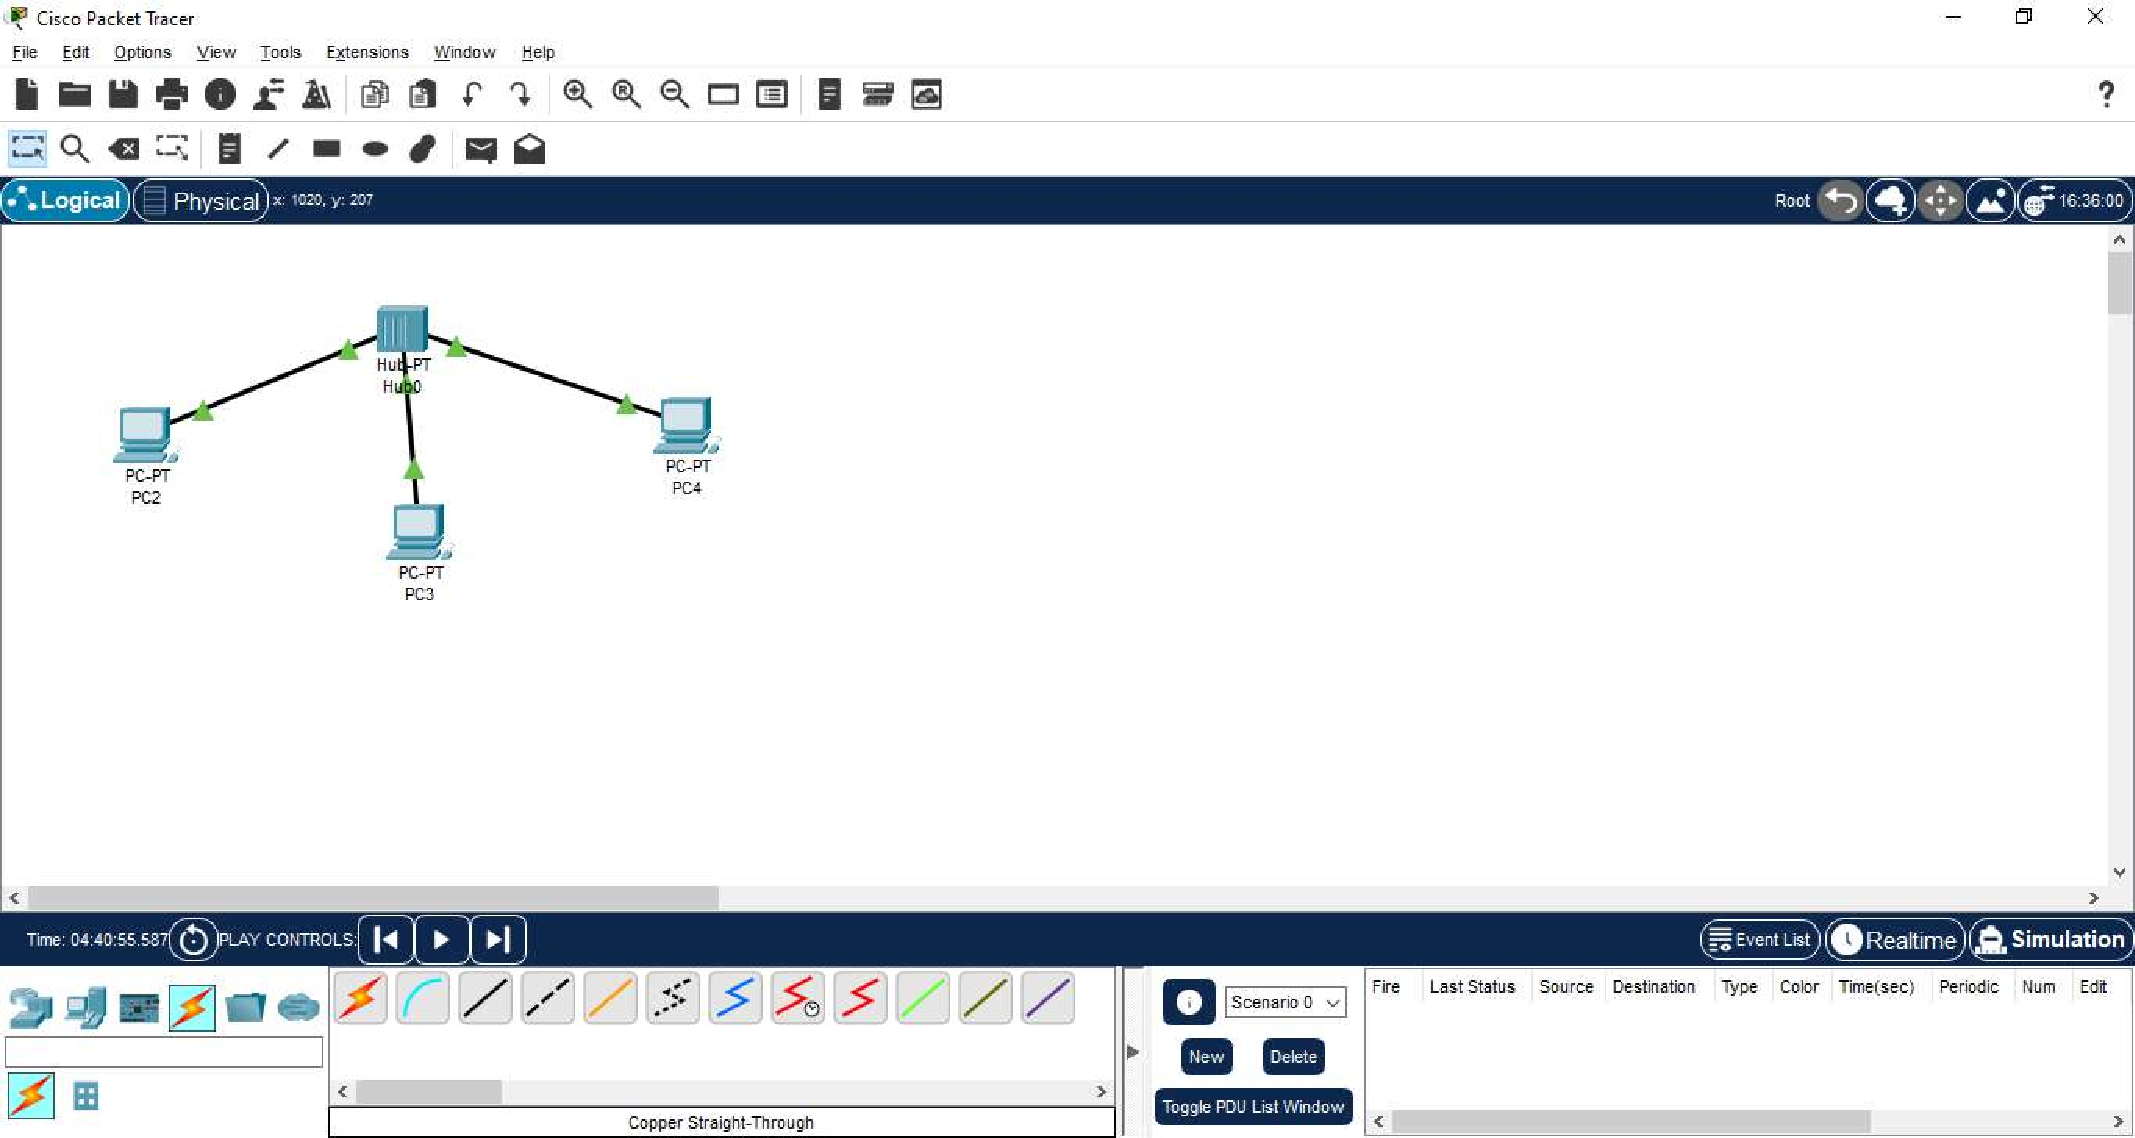
\includegraphics[width=.99\textwidth]{Figuras/hub}
    \caption{Topologia de barramento com hub.}
    \label{fig:hub}
\end{figure}

\subsection{Troca de dados entre os computadores}\label{subsec:trocaPDUs}
Veremos agora a troca de dados entre os nós (computadores) de uma rede. Chamaremos esses dados de \textit{Protocol Data Unit} (PDU). Na verdade, a PDU é a unidade básica de troca entre entidades que se comunicam usando um protocolo de rede específico.

Para simular o envio de PDUs usando a topologia de barramento, vamos executar os seguintes passos.

\begin{enumerate}[label*=\arabic*.]\label{enum:envioPDU}
    \item Selecione uma PDU simples, representada pelo ícone \faIcon[regular]{envelope} na barra de ferramentas. Você verá que o ponteiro do \textit{mouse} mudou para o mesmo ícone. Agora, você vai determinar a origem e o destino do PDU.
    \begin{enumerate}[label*=\arabic*.]
        \item Leve o ponteiro do \textit{mouse} a um dos PCs (por exemplo, o \texttt{PC0}) e clique sobre ele. Essa será a origem.
        \item Depois, leve o ponteiro do \textit{mouse} a outro dos PCs (por exemplo, o \texttt{PC2}) e clique sobre ele. Esse será o destino.
    \end{enumerate}
    
    \item Terminados os passos anteriores, vamos à simulação. Clique no botão de simulação (\textit{Simulation}) no canto inferior direito.

    \item Na nova janela que se abrir, clique no ícone \textit{play} (\faPlay) para rodar a simulação e observe o que acontece.
    \begin{enumerate}[label*=\arabic*.]
        \item Note que o PDU saiu da origem e foi encaminhado para todos os nós da rede. Porém, apenas o nó de destino confirmou seu reconhecimento (\textit{acknowledge}).
        \item O PDU de reconhecimento também foi enviado a todos os nós, mas apenas o nó destino o recebeu corretamente. Os demais nós descartaram a PDU que não era para eles.
     \end{enumerate}
\end{enumerate}

\section{Conexão de vários computadores com um \textit{switch}}\label{sec:conexSwitch}
Agora, vamos substituir o \textit{hub} por um \textit{switch}, para criar uma rede local com topologia estrela. Execute os passos a seguir.

\begin{enumerate}[label*=\arabic*.]
        \item Remova o \textit{hub}, clicando no ícone \faIcon{backspace} na barra de ferramentas e, em seguida, clicando sobre o \textit{hub}.
        \item No canto inferior esquerdo, dentre os dispositivos de rede (\textit{Network Devices}), selecione os \textit{switches}. Dentre os \textit{switches}, selecione o 2960.
        \item Agora, para cada um dos computadores, usando os cabos par trançados, execute os seguintes passos:
          \begin{enumerate}[label*=\arabic*.]
            \item Ligue a interface \textit{Fast Ethernet} do computador à interface \texttt{Fast Ethernet0/?} do \textit{switch}. Note que o 0 significa a VLAN 0. No lugar da `?', substitua por um número diferente (indicando que é outra interface do \textit{switch}).

            \item Aguarde um tempo até que o \textit{switch} resolva todas as conexões.

            \item Verifique se os computadores ainda estão com os mesmos endereços IP configurados (\texttt{10.0.0.5}, \texttt{10.0.0.6} e \texttt{10.0.0.7}) e máscara \texttt{255.0.0.0}.

            \item Verifique se todos os computadores estão visíveis entre si com o comando \Comando{ping}.
          \end{enumerate}
\end{enumerate}

Depois de terminada a configuração, repita a simulação descrita na \Cref{subsec:trocaPDUs}.

\section{Exercício}
Terminada as simulações nas \Cref{sec:conexHub,sec:conexSwitch}, quais foram as diferenças entre ambas as simulações?  O que acontece com as PDUs original e \textit{acknowledge} nas redes?  Por que dizemos que uma rede local interligada com um \textit{switch} tem uma topologia estrela?

\chapter{Criação de redes locais}\label{chp:redesCompletas}
%%%% Baseado na https://www.youtube.com/watch?v=2gva8vJpHD0
Agora que já conhecemos como criar uma rede simples, passaremos a criar uma rede local um pouco mais complexa. Essa rede local terá componentes cabeados e componentes sem fio (\textit{wireless}). Além disso, introduziremos o uso do \textit{Dynamic Host Configuration Protocol} (DHCP). O DHCP é um protocolo de serviço TCP/IP que oferece configuração dinâmica de terminais, com a atribuição dinâmica de endereços IP e máscara de sub-rede, \textit{gateway} padrão, número IP de um ou mais servidores DNS e sufixos de pesquisa do DNS, entre outras informações.

\section{Topologia da Rede local}\label{sec:testeSec}
Na topologia que vamos criar, ilustrada na \Cref{fig:topDHCP}, utilizaremos os seguintes equipamentos:
\begin{itemize}
    \item Quatro PCs, três \textit{laptops} e uma impressora.
    \item Um \textit{switch} (2960-24T) que vai conectar três dos cinco PCs e a impressora.
    \item Um roteador sem fio (\textit{wireless router} WRT300N) para conectar dois dos cinco PCs e os \textit{laptops} (sem fio).
\end{itemize}

\begin{figure}[!hbt]
    \centering
    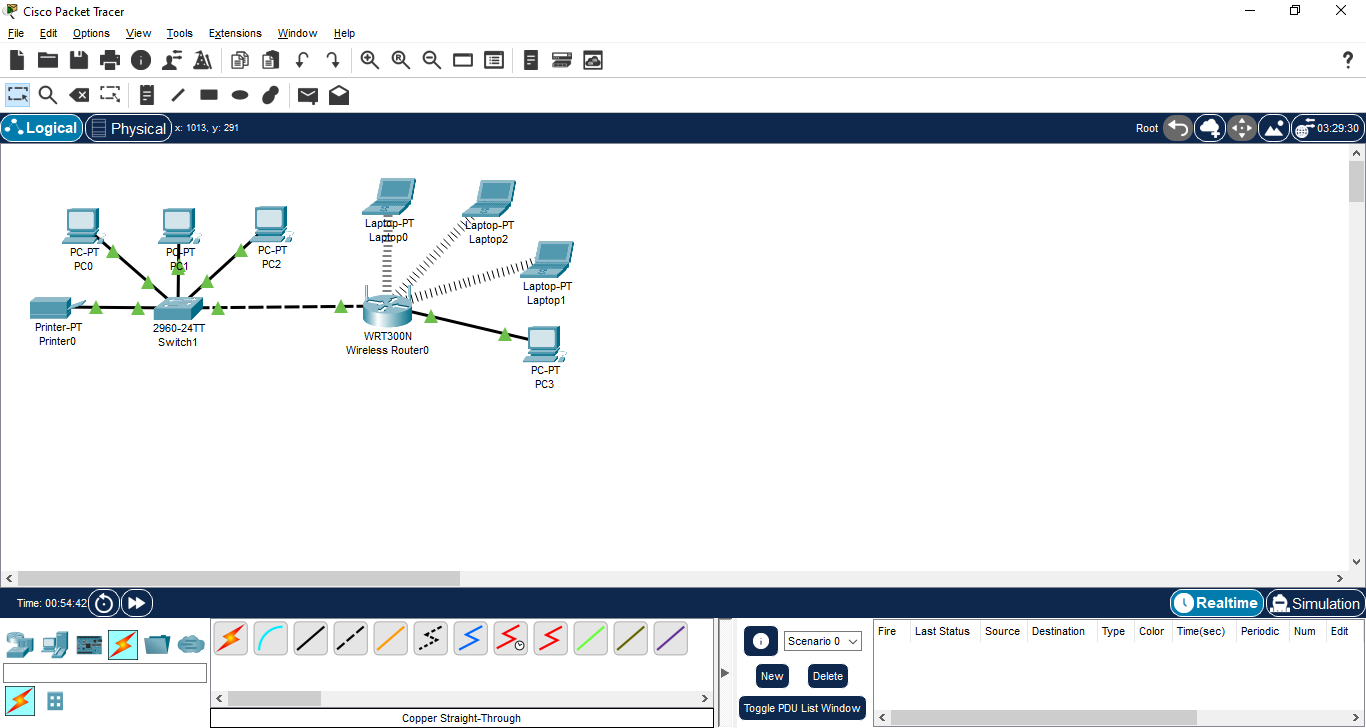
\includegraphics[width=.99\textwidth]{Figuras/RedeCompleta1}
    \caption{Topologia para rede local com DHCP.}\label{fig:topDHCP}
\end{figure}

Agora, vamos configurar essa rede local para que os equipamentos usem o DHCP para configuração automática dos seus endereços. Lembrando que  a impressora deve ter um IP fixo (\texttt{192.168.0.10}) e os demais equipamentos devem ter endereços dinâmicos atribuídos pelo DHCP.

Antes de começar, verifique se o cabeamento entre o \textit{switch} e o roteador sem fio é feito com um cabo \textit{cross-over}. Certifique-se também que os \textit{laptops} tenham placas para rede sem fio. Eles devem usar o módulo PT-LAPTOP-NM-1W-AC. Para instalar esse módulo (placa de rede) em um \textit{laptop}, execute os passos a seguir e observe a \Cref{fig:perfilLaptop}:

\begin{enumerate}[label*=\arabic*.]
  \item Clique sobre o ícone do \textit{laptop}.
  \item Na aba \textit{Physical}, você verá o perfil do \textit{laptop}. Desligue o equipamento, clicando no botão de liga/desliga (no canto esquerdo inferior da figura do \textit{laptop}).
  \item Arraste a placa de rede para a lista de módulos no canto esquerdo.
  \item Na lista de módulos, selecione o módulo PT-LAPTOP-NM-1W-AC e arraste para o local onde estava a placa de rede no \textit{laptop}.
\end{enumerate}

\begin{figure}[!hbt]
    \centering
    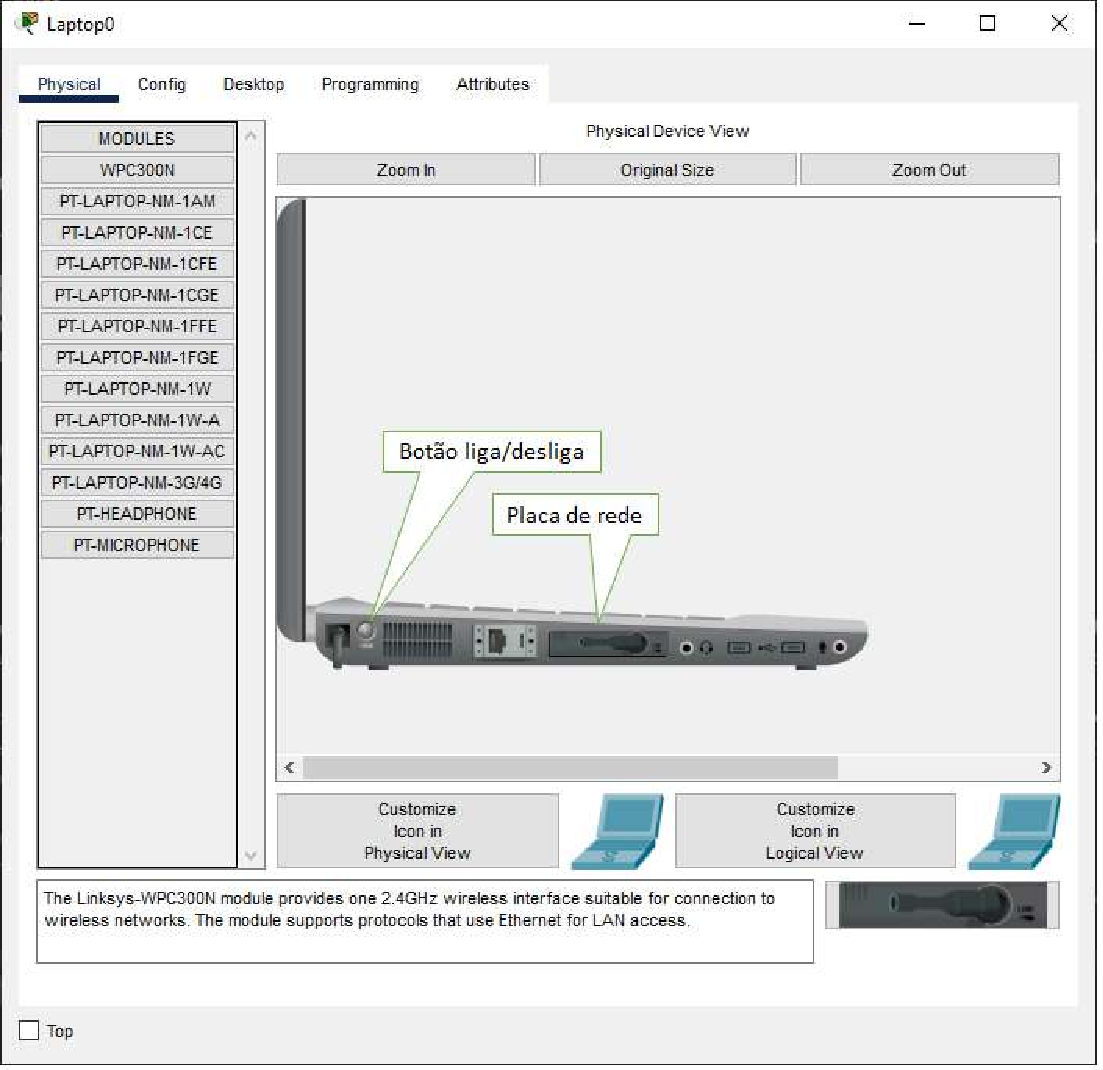
\includegraphics[scale=.8]{Figuras/PerfilLaptop}
    \caption{Perfil do \textit{laptop} para substituição da placa de rede sem fio.}\label{fig:perfilLaptop}
\end{figure}

\section{Configuração do roteador sem fio com DHCP}
Em redes sem fio, a utilização do DHCP é geralmente necessária, pois muitas vezes, há vários equipamentos que vão se ligar a essa rede. Assim, os equipamentos poderão ter suas configurações realizadas automaticamente. Realizaremos a seguir a configuração do DHCP no próprio roteador sem fio WRT300N. Os passos são os seguintes:

\begin{enumerate}[label*=\arabic*.]
  \item Clique sobre o ícone do roteador sem fio WRT300N.
  \item Na aba GUI, você verá a configuração inicial. Certifique-se que está na aba \textit{Setup} e com a opção \textit{Automatic Configuration -- DHCP} em tela.
  \item Identifique o \texttt{IP Address} do roteador. Ele já deve estar com o endereço IP \texttt{198.0.0.1} e máscara \texttt{255.255.255.0}.
  \item Confirme que o \texttt{DHCP server} está habilitado (\textit{Enable}).
  \item Agora, defina o endereço IP inicial (por padrão se inicia em 100) e o número máximo de usuários. Com isso, todos os novos usuários terão seus IPs a partir do endereço especificado. 
\end{enumerate}

Não esqueça de clicar no botão \textit{Save Settings} na parte inferior da tela. Use a barra de rolagem para descer até o final da tela.

O próximo passo é a definição do nome do roteador. Para isso, clique na aba \textit{Wireless} e, na definição do \textit{Network Name} (SSID), informe o nome para a sua rede sem fio. Nesse exemplo, vamos usar o nome \semaspas{RedeSemFio}. A propósito, a sigla SSID significa \textit{Service Set IDentifier}. Clique no botão \textit{Save Settings} na parte inferior da tela.

Agora definiremos algumas informações sobre a segurança no roteador sem fio. Para isso, clique na aba \textit{Wireless Security} (bem abaixo da opção \textit{Security}). Em seguida, na caixa de opções \textit{Security Mode}, selecione a opção \texttt{WPA2 Personal}. Mantenha todas as configurações padrão, mas especifique uma senha. \underline{Note que essa é a senha que os dispositivos utilizarão para ingressar na sua rede sem fio}.

O ideal é que a senha seja bastante complexa para aumentar a segurança. Mas, por simplicidade, vamos definir uma senha fácil \semaspas{Password123}. Note que há diferenças entre as letras minúsculas e maiúsculas. Clique no botão \textit{Save Settings} na parte inferior da tela.

Note que na opção \textit{Administration} no topo à direita estão as informações para o gerenciamento do roteador. A primeira dessas informações é a senha do roteador (\textit{Router Password}). Trata-se da senha para acesso às configurações do roteador. O valor padrão para senha é \semaspas{admin}. Por questões de segurança, é importante alterar.

\subsection{Configuração dos \textit{laptops} para conectar ao roteador sem fio}
Note que os \textit{laptops} precisam se conectar ao roteador sem fio com a nova senha. Para isso, é preciso configurar a rede sem fio de cada um dos equipamentos. Para isso, execute os passos a seguir para cada um dos \textit{laptops}.

\begin{enumerate}[label*=\arabic*.]
  \item Verifique se o \textit{laptop} está ligado.
  \item Clique na aba \textit{Config}. Depois, na lateral esquerda, clique na interface \textit{Wireless}.
  \begin{enumerate}[label*=\arabic*.]
    \item No campo \texttt{SSID}, informe o nome do seu roteador sem fio: \semaspas{RedeSemFio}.
    \item Na área \textit{Authentication}, selecione a opção \texttt{WPÀ2-PSK} e, ao lado, no campo \texttt{PSK Pass Phrase} informe a senha  \semaspas{Password123}.
   \end{enumerate}
   \item Certifique-se que na parte inferior dessa janela, na seção \texttt{IP Configuration}, está selecionado o DHCP. 
\end{enumerate}

\section{Configuração dos PCs e da impressora com o \textit{switch}}\label{sec:PCsSwitchDHCP}
A instalação do \textit{switch}, dos PCs e da impressora é bastante simples. Usando um cabo par-trançado, conecte cada um dos PCs e a impressora ao \textit{switch}. Por sua vez, usando um cabo \textit{cross-over}, conecte a porta \texttt{FastEthernet0/24} do \textit{switch} ao roteador sem fio. Note que, nesse instante, todos os equipamentos estarão conectados entre si. Isso porque, por padrão, todos os equipamentos nessa simulação estão usando o DHCP.

Porém, lembre-se que optamos por definir um endereço IP fixo para a impressora (\texttt{192.168.0.10}). Portanto, precisamos fazer essa configuração específica. Execute os passos a seguir.

\begin{enumerate}[label*=\arabic*.]
  \item Clique na impressora. Depois, na janela que se abrir, clique na aba \textit{Config}.
  \begin{enumerate}[label*=\arabic*.]
    \item Na lateral esquerda, clique na opção \texttt{FastEthernet0}
  \end{enumerate}  
  \item Agora, na área \texttt{IP Configuration}, faça o seguinte:
  \begin{enumerate}[label*=\arabic*.]
     \item Selecione a opção \texttt{Static}.
     \item No campo \texttt{IPv4 Address}, informe o endereço \texttt{192.168.0.10}.
     \item No campo \texttt{Subnet Mask}, informe o endereço \texttt{255.255.255.0}.
  \end{enumerate}
\end{enumerate}

Se tudo deu certo, toda a rede deve estar conectada.

\section{Exercícios}\label{sec:ExercicioRedesComplexas}

Verifique se tudo está ok, enviando um PDU de um dos \textit{laptops} para a impressora. A sequência de passos para envio de um PDU de um dispositivo para outro está na \Cpageref{enum:envioPDU}.

Agora, verifique se um dos PCs ligados ao \textit{switch} consegue alcançar todos dos \textit{laptops} da rede sem fio. Para isso, execute as seguintes tarefas:

\begin{enumerate}[label*=\arabic*.]
\item Descubra os endereços IP dos três \textit{laptops} da sua rede.
\item Em um dos PCs, entre no \textit{prompt} de comando. 
\item Para cada um dos endereços IPs dos \textit{laptops} faça:
    \begin{enumerate}[label*=\arabic*.] 
       \item Execute o comando \Comando{ping} para o IP daquele \textit{laptop} escolhido.
    \end{enumerate}
\end{enumerate}

\chapter{Redes locais virtuais}\label{chp:vlan}
%%%% https://www.youtube.com/watch?v=H01eZjdcHTo
As redes locais virtuais (\textit{virtual local area networks} -- VLAN) é uma rede local que, embora esteja ligada fisicamente a partir de um mesmo equipamento (\textit{switch}, por exemplo), está segmentada logicamente em duas ou mais redes locais. Cada uma das redes locais lógicas é independente das demais, formando o que chamamos de \enquote{domínio de \textit{broadcast}}. Neste capítulo, vamos ver como configurar uma VLAN usando o \CPT. 

Para ilustrar, vamos supor que em uma instituição exemplo (uma universidade), temos três redes lógicas diferentes, conforme apresentado na \Cref{fig:vlan}. Assim, teremos uma rede lógica para docentes, outra para funcionários e uma terceira para estudantes.

\begin{figure}[!htb]
    \centering
    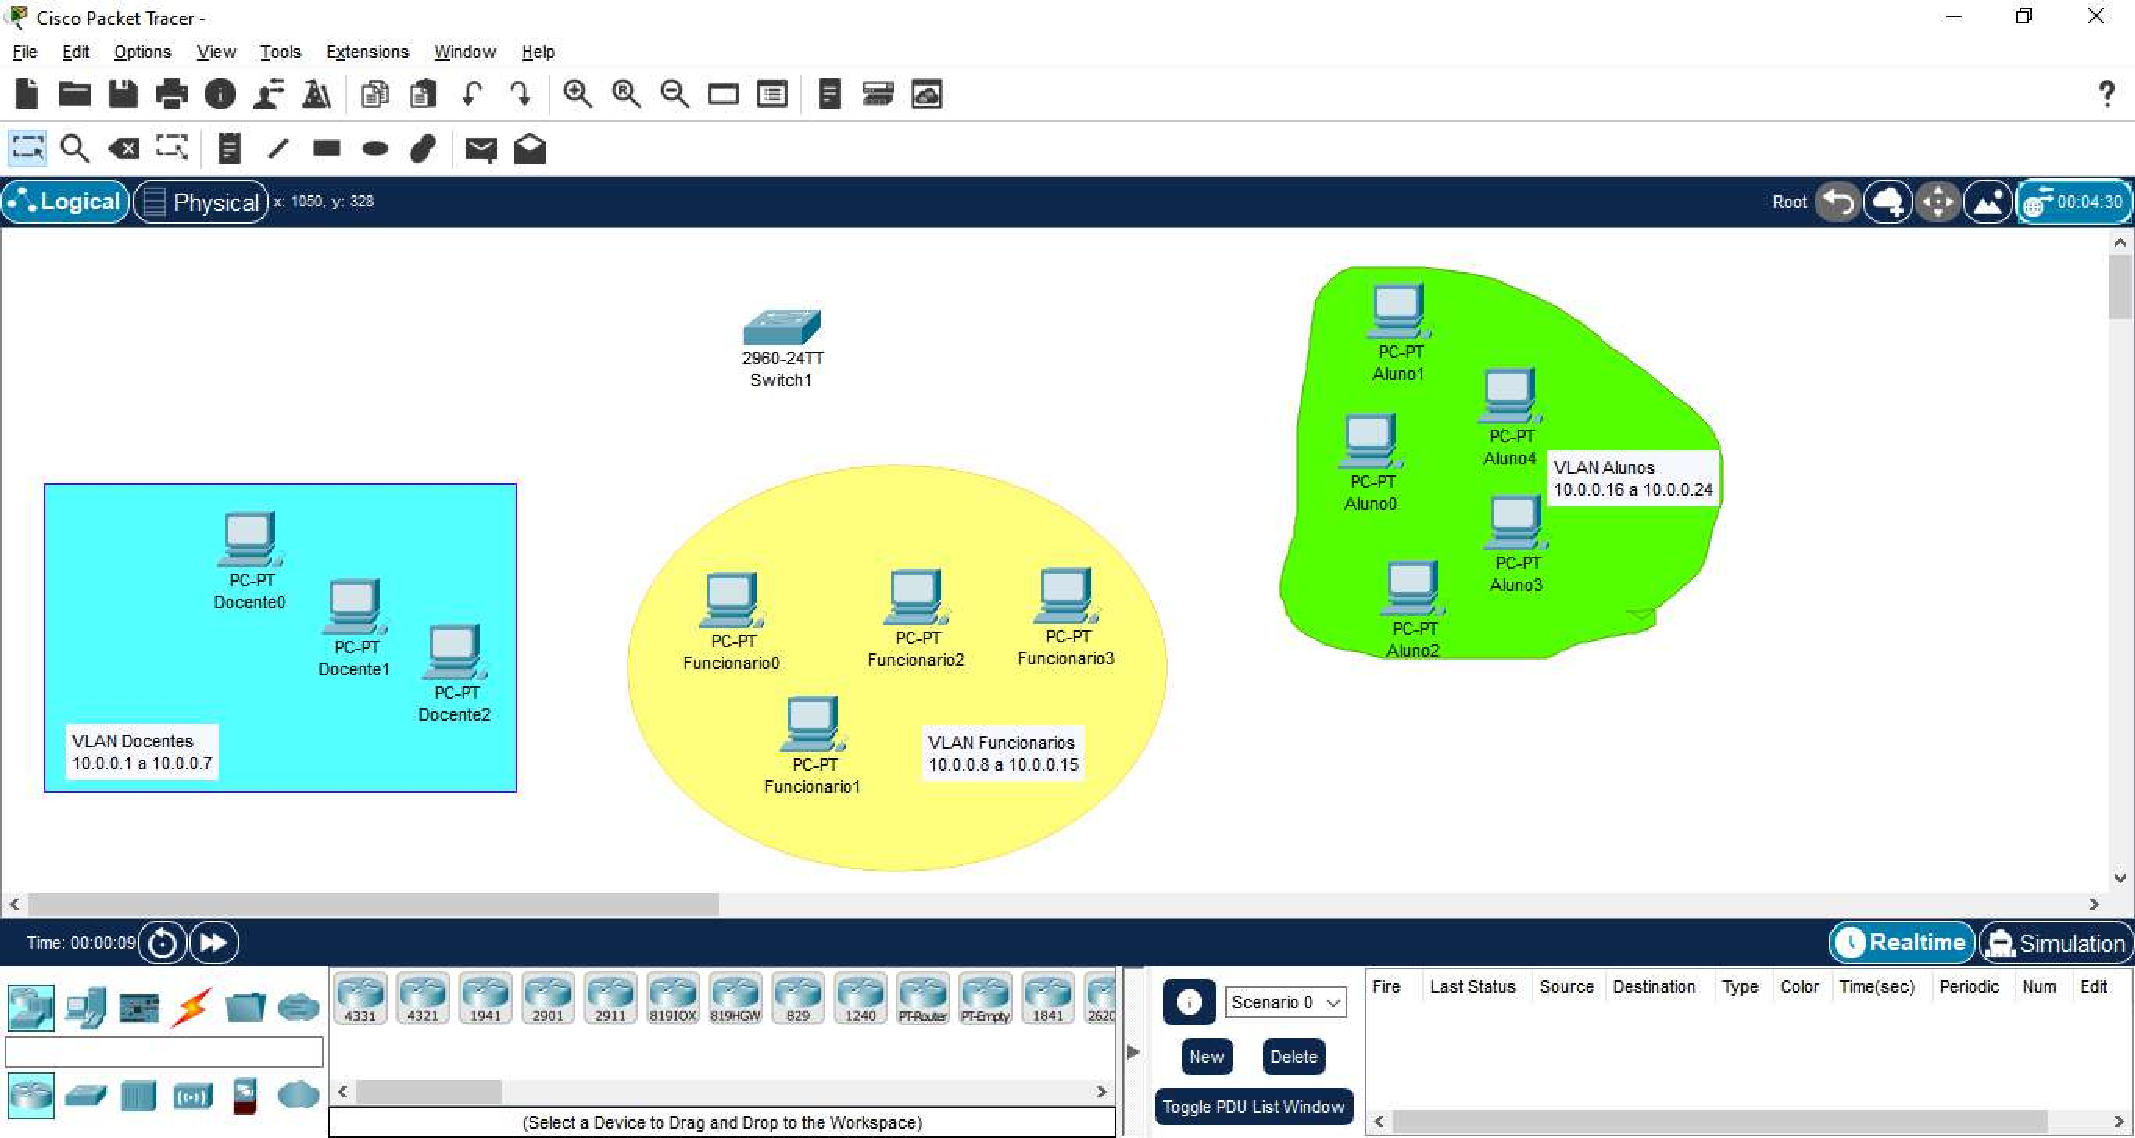
\includegraphics[width=.99\textwidth]{Figuras/vlan}
    \caption{VLANs diferentes em uma organização.}
    \label{fig:vlan}
\end{figure}

\section{Topologia das VLANs}\label{sec:topVLAN}
A topologia proposta para ilustrarmos a configuração de VLANs é a seguinte:
\begin{itemize}
    \item A VLAN para docentes, de início, terá três PCs conectados e terá reservados os endereços IP das faixas \texttt{10.0.0.1} a  \texttt{10.0.0.7}.
    \item A VLAN para funcionários, de início, terá quatro PCs conectados e terá reservados os endereços IP das faixas \texttt{10.0.0.8} a  \texttt{10.0.0.15}.
    \item A VLAN para alunos, de início, terá cinco PCs conectados e terá reservados os endereços IP das faixas \texttt{10.0.0.16} a  \texttt{10.0.0.24}.
\end{itemize}

Note que utilizaremos apenas um \textit{switch} de 24 portas (Modelo 2960) para estabelecer essas VLANs. Perceba também que dividimos oito endereços IPs para cada VLAN, embora não utilizaremos todos em um primeiro momento.

Antes de começar a configuração da VLAN, conecte todos os PCs ao \textit{switch}. \textbf{Atente para a divisão das 
interfaces entre as VLANs}. Dessa forma, faça o seguinte:
\begin{enumerate}[label*=\arabic*.]\label{enum:divInterfaces}
\item Para os PCs da VLAN dos docentes:
   \begin{enumerate}[label*=\arabic*.]
       \item Conecte a interface \texttt{FastEthernet0} do PC \texttt{Docente0} à interface \texttt{FastEthernet0/1} do \textit{switch}.
       \item Conecte a interface \texttt{FastEthernet0} do PC \texttt{Docente1} à interface \texttt{FastEthernet0/2} do \textit{switch}.
       \item Conecte a interface \texttt{FastEthernet0} do PC \texttt{Docente2} à interface \texttt{FastEthernet0/3} do \textit{switch}.
   \end{enumerate}
\item Para os PCs da VLAN dos funcionários:
   \begin{enumerate}[label*=\arabic*.]
       \item Conecte a interface \texttt{FastEthernet0} do PC \texttt{Funcionario0} à interface \texttt{Fast\-Ether\-net0/8} do \textit{switch}.
       \item Conecte a interface \texttt{FastEthernet0} do PC \texttt{Funcionario1} à interface \texttt{Fast\-Ether\-net0/9} do \textit{switch}.
       \item Conecte a interface \texttt{FastEthernet0} do PC \texttt{Funcionario2} à interface \texttt{Fast\-Ether\-net0/10} do \textit{switch}.
       \item Conecte a interface \texttt{FastEthernet0} do PC \texttt{Funcionario3} à interface \texttt{Fast\-Ether\-net0/11} do \textit{switch}.
   \end{enumerate}
\item Para os PCs da VLAN dos alunos:
   \begin{enumerate}[label*=\arabic*.]
       \item Conecte a interface \texttt{FastEthernet0} do PC \texttt{Aluno0} à interface \texttt{FastEthernet0/17} do \textit{switch}.
       \item Conecte a interface \texttt{FastEthernet0} do PC \texttt{Aluno1} à interface \texttt{FastEthernet0/18} do \textit{switch}.
       \item Conecte a interface \texttt{FastEthernet0} do PC \texttt{Aluno2} à interface \texttt{FastEthernet0/19} do \textit{switch}.
       \item Conecte a interface \texttt{FastEthernet0} do PC \texttt{Aluno3} à interface \texttt{FastEthernet0/20} do \textit{switch}.
       \item Conecte a interface \texttt{FastEthernet0} do PC \texttt{Aluno4} à interface \texttt{FastEthernet0/21} do \textit{switch}.
   \end{enumerate}
\end{enumerate}

Aguarde um tempo e verá que todas as comunicações estão funcionando. 

\section{Exercício}
Agora, como teste, verifique se consegue enviar um PDU de um computador da rede \texttt{alunos} para a rede \texttt{docentes}.

Se tudo funcionou bem, perceba que todos os PCs estão em uma mesma rede local. Portanto, todos são acessíveis entre si.

\section{Configuração das VLANs}\label{sec:configVLAN}
Agora vamos configurar cada uma das VLANs. Por uma questão de organização, vamos nomeá-las de \texttt{VLANDocentes}, \texttt{VLANFuncionários} e \texttt{VLANAlunos}, respectivamente.

Toda a configuração será feita no \textit{switch}. Para configurar o \textit{switch}, precisamos acessar a interface da linha de comando (\textit{Command Line Interface} -- CLI). Para isso, clique sobre o \textit{switch} e, depois, selecione a aba \texttt{CLI}.

Ao selecionar a aba \texttt{CLI}, você estará na console de configuração do \textit{switch}. Tecle \keys{\enter} e o \textit{prompt} com a \textit{string} \enquote{\texttt{Switch>}} mostrará que está pronto para receber os comandos. Agora execute os passos a seguir.

\begin{enumerate}[label*=\arabic*.]
    \item Digite \semaspas{enable} para entrar no modo administrador. Note que o \textit{prompt} mudou para \enquote{\texttt{Switch\#}}.
    \item Digite \semaspas{configure terminal} para entrar na configuração global\footnote{Você também pode digitar apenas as primeiras letras do comando. Por exemplo, você poderá digitar apenas \semaspas{conf term} para entrar na configuração global.}. Note que o \textit{prompt} mudou para \enquote{\texttt{Switch (config)\#}}.
    \item Agora defina o número (inteiro) da VLAN que você vai criar. Lembre-se que a \texttt{VLAN 1} é a VLAN \textit{default}. Portanto, as demais VLANs devem começar a partir de \texttt{2}. Assim, para cada VLAN, começando da VLAN 2, vamos executar os passos a seguir:
    
    \begin{enumerate}[label*=\arabic*.]
        \item Digite \semaspas{VLAN X} para entrar na configuração da VLAN X, onde X pode ser 2 (para a rede de docentes), 3 (para a rede de funcionários) ou 4 (para a rede de alunos).
        \item Note que o \textit{prompt} mudou para  \enquote{\texttt{Switch (config-vlan)\#}}. Agora digite o comando a seguir  para atribuir um nome à VLAN que você está configurando. Não esqueça de substituir \texttt{nome\_da\_vlan} pelo nome da respectiva VLAN que você está configurando (\texttt{VLANDocentes}, \texttt{VLANFuncionários} ou \texttt{VLANAlunos}).

        \texttt{\textcolor{green}{Switch(config-vlan)\#} \textcolor{blue}{name} nome\_da\_vlan}

        \item Digite \semaspas{exit} para encerrar a configuração dessa VLAN.
    \end{enumerate}

    \item Depois de terminar todas as configurações de VLANs, digite \semaspas{exit} para encerrá-las.
    
    \item Verifique que todas as VLANs foram criadas com o comando a seguir:  

       \texttt{\textcolor{green}{Switch\#} \textcolor{blue}{show} vlan brief}

    Note que as VLANS já existem, mas ainda não há  interfaces (portas) atribuídas a elas.
       
    \item Agora, vamos atribuir as respectivas portas para cada VLAN. Primeiro, digite \semaspas{conf term} para entrar na configuração global.

    \item Para cada interface, vamos executar os passos a seguir. Lembre-se da divisão das interfaces que fizemos na \Cpageref{enum:divInterfaces}.

       \begin{enumerate}[label*=\arabic*.]
          \item Digite o comando \semaspas{int F0/Y}, substituindo o \texttt{Y} pelo número da interface que você quer configurar.
          \item Digite o comando \semaspas{switchport access VLAN X}, substituindo o \texttt{X} pelo número da VLAN à qual você quer atribuir aquela interface. 
          
          É importante lembrar que, ao pressionar a tecla \keys{\arrowkey{^}} (seta para cima), a CLI repete o último comando.
       \end{enumerate}
    
    \item Depois de configuradas todas as interfaces, digite \semaspas{end} para sair. Ou, se preferir, digite \keys{\ctrl+z} para voltar à raiz do CLI.

    \item Use o comando \semaspas{show vlan brief} para verificar se a distribuição das portas (interfaces) às respectivas VLANs está ok.

    \item Agora digite o comando \semaspas{write} para gravar as alterações. 
\end{enumerate}

\section{Exercício}
Agora, como teste, verifique se as os PCs dentro de uma VLAN são acessíveis entre si. Envie um PDU de um PC em uma VLAN para outro PC na mesma VLAN.

Depois, verifique se você consegue enviar um PDU de um PC em uma VLAN para outro PC em outra VLAN.

\chapter{Redes de longa distância}\label{chp:roteamento}
%%% https://www.dailymotion.com/video/x11vklx
%%% https://www.youtube.com/watch?v=YdM7yBrtAck
Neste capítulo, vamos ligar duas redes locais para formar uma rede de longa distância (\textit{Wide Area Network} -- WAN). Para isso, as redes locais, que já estão interconectadas com \textit{switches}, vão utilizar os roteadores para se interconectar. Utilizaremos como base a estrutura ilustrada na \Cref{fig:roteamentoInicio} a seguir.

\begin{figure}[!hbt]
    \centering
    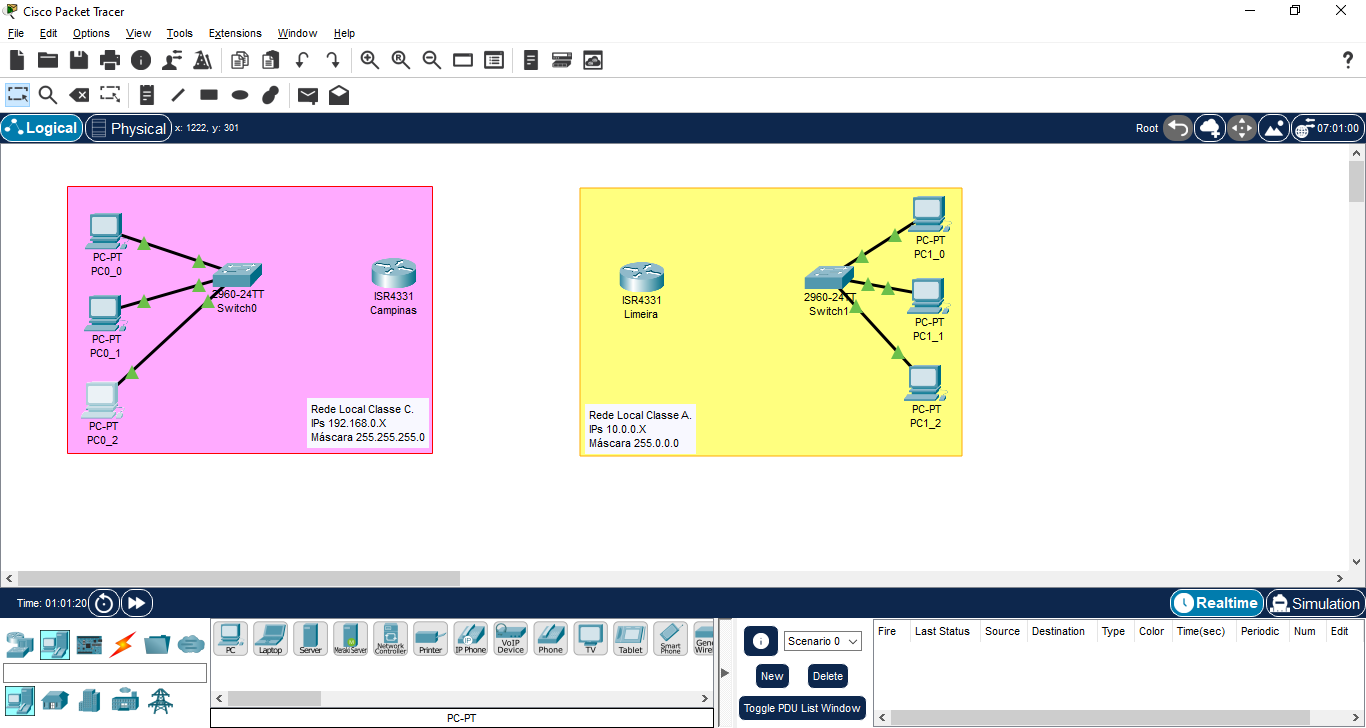
\includegraphics[width=.99\textwidth]{Figuras/InterRedesLocais}
    \caption{Redes locais que serão interligadas.}\label{fig:roteamentoInicio}
\end{figure}

De início, as redes locais da esquerda e da direita, ilustrada na \Cref{fig:roteamentoInicio}, são compostas, cada uma, por três PCs interligados a um \textit{switch} (Modelo 2960) com cabos par-trançados. Posteriormente, adicionaremos um roteador (modelo ISR 4331) em cada uma das redes e os interligaremos. Estamos supondo que a rede da esquerda está fisicamente em Campinas e a rede da direita está fisicamente em Limeira.

A rede da esquerda é uma rede local classe C. Portanto, os endereços IP estáticos são \texttt{192.168.0.X}, onde \texttt{X} é substituído por \texttt{2} no \texttt{PC0\_0}, \texttt{3} no \texttt{PC0\_1} e \texttt{4} no \texttt{PC0\_2}. A máscara em todos os PCs dessa rede é \texttt{255.255.255.0}. 

De forma análoga, a  rede da direita é uma rede local classe A. Portanto, os endereços IP estáticos são \texttt{10.0.0.X}, onde \texttt{X} é substituído por \texttt{2} no \texttt{PC1\_0}, \texttt{3} no \texttt{PC1\_1} e \texttt{4} no \texttt{PC1\_2}. A máscara em todos os PCs dessa rede é \texttt{255.0.0.0}. 

Certifique-se que as redes locais estejam funcionando normalmente antes de proceder com os próximos passos.

\section{Conexão da rede local a um roteador}\label{sec:conexaoRedeLocalRoteador}
Em cada uma das redes locais, vamos adicionar um roteador (modelo ISR 4331) e, posteriormente, ligá-lo a sua rede local com um cabo par trançado. A ligação será feita usando a porta \texttt{Gi\-ga\-bit\-Ether\-net\-0/1} do \textit{switch} à porta \texttt{Gi\-ga\-bit\-Ether\-net\-0/0/0} do roteador. O mesmo procedimento deverá ser feito para cada rede local. Para diferenciar os roteadores de cada rede local, vamos nomeá-los de \texttt{Campinas} e \texttt{Limeira}, respectivamente. 

Note que a conexão física está estabelecida, mas ainda não há transmissão de dados entre os roteadores. Então, precisamos configurá-los.

\subsection{Configuração dos roteadores para conexão com a LAN}\label{subsec:configRoreadores}
Para configurar cada um dos roteadores, precisamos acessar a interface da linha de comando (CLI). Para isso, clique em um dos roteadores e, depois, selecione a aba \texttt{CLI}.

Uma janela aparecerá, perguntando se você quer entrar na configuração do roteador (\textit{Would you like to enter basic management setup? [yes/no]}). Digite \semaspas{no} e pressione \keys{\enter}. O \textit{prompt} com a \textit{string} \enquote{\texttt{Router>}} mostrará que está pronto para receber os comandos. Agora execute os passos a seguir.

\begin{enumerate}[label*=\arabic*.]
    \item Digite \semaspas{enable} para entrar no modo administrador. Note que o \textit{prompt} mudou para \enquote{\texttt{Router\#}}.
    \item Digite \semaspas{conf terminal} para entrar na configuração global. Note que o \textit{prompt} mudou para \enquote{\texttt{Router (config)\#}}.
    \item Agora defina o nome do roteador. Para isso, digite \semaspas{hostname Campinas} para definir o nome desse roteador. Note que para o outro roteador, você deverá atribuir outro nome (\texttt{Limeira}).
    \item Verifique se as configurações até o momento estão de acordo. Para isso execute os seguintes passos:
    \begin{enumerate}[label*=\arabic*.]
        \item Digite \semaspas{exit} para sair do modo configuração.
        \item Digite \semaspas{show running-config} para mostrar a configuração até o momento.
    \end{enumerate}
\end{enumerate}

Note que o \texttt{hostname} está configurado, mas as interfaces \textit{GigabitEthernet} não têm endereços IP atribuído a elas e também estão desligadas (\texttt{shutdown}). Vamos então, configurar a conexão entre o roteador (\texttt{Campinas}) à sua rede local. Para tanto, execute  os próximos passos ainda na CLI.

\begin{enumerate}[label*=\arabic*.]
    \item Digite novamente \semaspas{conf terminal} para entrar na configuração global. 
    \item Digite \semaspas{interface GigabitEthernet 0/0/0} para configurar a interface à qual o \textit{switch} está conectado.
    \item Atribua o IP e a máscara à essa interface com o comando a seguir:
    
       \texttt{\textcolor{green}{Campinas(config-if)\#} \textcolor{blue}{ip} address 192.168.0.1 255.255.255.0}

    \item Em seguida, ligue a porta e a mantenha ligada com o comando \semaspas{no shutdown}.
    \item Por uma questão de organização, vamos atribuir uma descrição para essa interface com o comando \Comando{description}. Note que, após o comando, vem a descrição daquela interface. Usaremos o comando a seguir:
    
       \texttt{\textcolor{green}{Campinas(config-if)\#} \textcolor{blue}{description} Porta LAN Campinas}
       
    \item Verifique se as configurações até o momento estão de acordo. Para isso execute os seguintes passos:
    \begin{enumerate}[label*=\arabic*.]
        \item Digite \semaspas{exit}  duas vezes para sair do modo de configuração da interface e do modo de configuração global.
        \item Digite \semaspas{show running-config} para mostrar a configuração até o momento.
    \end{enumerate}
\end{enumerate}

Repita o mesmo procedimento para o roteador em Limeira. Note que o endereço IP do roteador será \texttt{10.0.0.1} e a máscara \texttt{255.0.0.0}.

\section{Conexão dos roteadores entre si}\label{subsec:conexaoRoteadores}
Depois que cada rede local está conectada ao seu respectivo roteador, vamos conectar os roteadores entre si. Nós utilizaremos um cabo par trançado e conectaremos ambos os roteadores nas respectivas portas \texttt{Gi\-ga\-bit\-Ether\-net\-0/0/1}.

É importante lembrar que teremos, conceitualmente, três redes: LAN de Campinas (\texttt{192.168.0.0}), a LAN de Limeira (\texttt{10.0.0.0}) e a WAN que interliga ambas as redes (\texttt{200.100.10.0}). Para a WAN, definimos que os roteadores terão os IPs \texttt{200.100.10.1} para Campinas e \texttt{200.100.10.2} para Limeira, ambas com a máscara \texttt{255.255.255.0}. 

Para a configuração dos roteadores, será preciso executar os passos a seguir. Faremos inicialmente no roteador que está em \texttt{Campinas}.
\begin{enumerate}[label*=\arabic*.]
  \item Entre novamente na interface da linha de comando do roteador (veja detalhes no início da \Cref{subsec:configRoreadores}).
  \item Digite \semaspas{enable} para entrar no modo administrador. 
  \item Digite \semaspas{conf terminal} para entrar na configuração global.
  \item Defina a interface que será configurada. Nesse caso, vamos usar a interface que liga este roteador ao roteador de \texttt{Limeira}. Use o comando a seguir:

    \texttt{\textcolor{green}{Campinas(config)\#} \textcolor{blue}{interface} GigabitEthernet0/0/1}
  
  \item Atribua o IP e a máscara à essa interface e informe que a interface estará ativa com os comandos a seguir. Note que geralmente esses IP e máscara são atribuídos por uma empresa de telecomunicações, responsável pela rede de longa distância. Nesse exemplo, usaremos o IP \texttt{200.100.10.1} com a máscara \texttt{255.255.255.0}.
    
       \texttt{\textcolor{green}{Campinas(config-if)\#} \textcolor{blue}{ip} address 200.100.10.1 255.255.255.0}

       \texttt{\textcolor{green}{Campinas(config-if)\#} \textcolor{blue}{no shutdown}}

   \item Por uma questão de organização, vamos atribuir uma descrição para essa interface com o comando \Comando{description}. Note que, após o comando, vem a descrição daquela interface. Usaremos o comando a seguir:
    
       \texttt{\textcolor{green}{Campinas(config-if)\#} \textcolor{blue}{description} Porta WAN Campinas-Limeira}

   \item Para uma configuração mais precisa, vamos usar o comando \Comando{bandwidth} para estabelecer a largura de banda dessa conexão. Como é uma \textit{Gigabit Ethernet}, vamos estabelecer uma largura de banda de 125.000.000 \textit{bytes} por segundo (Bps). Para isso, usamos o comando a seguir. Perceba que o valor está em \textit{kilobytes}. Portanto, 125.000.000 bytes por segundo é 125000 \textit{kilobytes} por segundo (KBps).
   
       \texttt{\textcolor{green}{Campinas(config-if)\#} \textcolor{blue}{bandwidth} 125000}

  \item Saia da configuração da interface com o comando \semaspas{exit} e vamos configurar o protocolo de roteamento \textit{Routing Information Protocol} (RIP) com o comando a seguir. Note que poderíamos usar outros protocolos como o \textit{Border Gateway Protocol} (BGP), \textit{Enhanced Interior Gateway Routing Protocol} (EIGRP) ou \textit{Open Shortest Path First} (OSPF).

        \texttt{\textcolor{green}{Campinas(config)\#} \textcolor{blue}{router} rip}
  
  \begin{enumerate}[label*=\arabic*.]
    \item Note que o \textit{prompt} mudou para \enquote{\texttt{Campinas(config-router)\#}}. Agora, vamos informar as três redes às quais o roteador está conectado com os comandos a seguir. 

        \texttt{\textcolor{green}{Campinas(config-router)\#} \textcolor{blue}{network} 192.168.0.0}

        \texttt{\textcolor{green}{Campinas(config-router)\#} \textcolor{blue}{network} 10.0.0.0}

        \texttt{\textcolor{green}{Campinas(config-router)\#} \textcolor{blue}{network} 200.100.10.0}

    \item Volte à configuração do terminal digitando o comando \Comando{exit} e pressionando a tecla \keys{\enter} \underline{duas vezes}. Eventualmente, você poderá digitar \semaspas{end} ou simplesmente pressionar \keys{\ctrl + Z}.
  \end{enumerate}
  
  \item Note que todas essas configurações estão na memória, mas não foram salvas. Para salvá-las de forma permanente, use o comando a seguir e pressione \keys{\enter} em seguida:

       \texttt{\textcolor{green}{Campinas\#} \textcolor{blue}{copy} running-config startup-config}
  \begin{enumerate}[label*=\arabic*.]
    \item Confirme que a configuração foi salva usando o comando a seguir:

      \texttt{\textcolor{green}{Campinas\#} \textcolor{blue}{show} startup-config}
  \end{enumerate}
\end{enumerate}

Agora, basta repetir o mesmo procedimento para o roteador em \texttt{Limeira}. Não esqueça de substituir os endereços e máscaras das respectivas redes. A lista de comandos a serem executados no roteador de Limeira é a seguinte:
\begin{itemize}
    \item \texttt{\textcolor{green}{Campinas(config-if)\#} \textcolor{blue}{interface} GigabitEthernet0/0/1}
    \item \texttt{\textcolor{green}{Router>} \textcolor{blue}{enable}}
\item \texttt{\textcolor{green}{Router\#} \textcolor{blue}{conf} terminal}
\item \texttt{\textcolor{green}{Router(config)\#} \textcolor{blue}{hostname} Limeira}
\item \texttt{\textcolor{green}{Limeira(config)\#} \textcolor{blue}{interface} GigabitEthernet 0/0/0}
\item \texttt{\textcolor{green}{Limeira(config-if)\#} \textcolor{blue}{ip} address 10.0.0.1 255.0.0.0}
\item \texttt{\textcolor{green}{Limeira(config-if)\#} \textcolor{blue}{no} shutdown}
\item \texttt{\textcolor{green}{Limeira(config-if)\#} \textcolor{blue}{description} Porta LAN Limeira}
\item \texttt{\textcolor{green}{Limeira(config-if)\#} \textcolor{blue}{exit}}
\item \texttt{\textcolor{green}{Limeira(config)\#} \textcolor{blue}{interface} GigabitEthernet0/0/1}
\item \texttt{\textcolor{green}{Limeira(config-if)\#} \textcolor{blue}{ip} address 200.100.10.2 255.255.255.0}
\item \texttt{\textcolor{green}{Limeira(config-if)\#} \textcolor{blue}{no} shutdown}
\item \texttt{\textcolor{green}{Limeira(config-if)\#} \textcolor{blue}{description} Porta WAN Limeira-Campinas}
\item \texttt{\textcolor{green}{Limeira(config-if)\#} \textcolor{blue}{bandwidth} 125000}
\item \texttt{\textcolor{green}{Limeira(config-if)\#} \textcolor{blue}{exit}}
\item \texttt{\textcolor{green}{Limeira(config)\#} \textcolor{blue}{router} rip}
\item \texttt{\textcolor{green}{Limeira(config-router)\#} \textcolor{blue}{network} 192.168.0.0}
\item \texttt{\textcolor{green}{Limeira(config-router)\#} \textcolor{blue}{network} 10.0.0.0}
\item \texttt{\textcolor{green}{Limeira(config-router)\#} \textcolor{blue}{network} 200.100.10.0}
\item \texttt{\textcolor{green}{Limeira(config-router)\#} \textcolor{blue}{exit}}
\item \texttt{\textcolor{green}{Limeira\#} \textcolor{blue}{exit}}
\item \texttt{\textcolor{green}{Limeira\#} \textcolor{blue}{copy} running-config startup-config}
\end{itemize}

Confirme que todos os computadores estão de fato conectados, executando o \Comando{ping} de um computador na rede de Limeira, para o IP de um computador que está na rede de Campinas.

\section{Exercício}
Adicione a rede atual mais uma rede Local em Piracicaba. Em seguida, adicione um roteador à rede de Piracicaba e interligue-o aos demais roteadores. Faça as devidas configurações e teste para ver se todas as redes estão alcançáveis entre si.

\section{Configuração de roteadores com DHCP}
Ao configurar as redes de longa distância anteriores, nós definimos um endereço IP fixo para todos os computadores. No entanto, a utilização do DHCP permitirá a adição de novos computadores à rede local, sem que seja necessário se preocupar com a configuração manual dos endereços IP.

Para isso, escolha um dos roteadores (nesse exemplo, escolheremos o roteador de Limeira), clique sobre ele e entre na CLI. Depois, execute os passos a seguir:

\begin{enumerate}[label*=\arabic*.]
   \item Digite \semaspas{enable} para entrar no modo administrador.
   \item Digite \semaspas{conf terminal} para entrar na configuração global.
   \item Crie e nomeie um \textit{pool} (agrupamento) de endereços IP que serão atribuídos pelo DHCP com o comando a seguir. Nesse caso, o nome que utilizaremos será \texttt{dhcpLimeira}.

    \texttt{\textcolor{green}{Limeira(config)\#} \textcolor{blue}{ip} ip dhcp pool dhcpLimeira}

   \item Para garantir, vamos definir a rede padrão com os comandos a seguir: 
   
     \texttt{\textcolor{green}{Limeira(dhcp-config)\#} \textcolor{blue}{network} 10.0.0.0 255.0.0.0}
     
     \texttt{\textcolor{green}{Limeira(dhcp-config)\#} \textcolor{blue}{default-router} 10.0.0.1}

    \item Agora, vamos excluir uma faixa de endereços IP do \textit{pool}, que vai de \texttt{10.0.0.1} a \texttt{10.0.0.9}. Isso é necessário para garantir que o roteador e alguns outros endereços IPs não sejam atribuídos pelo DHCP. Com isso, evitamos colisões do roteador com outros IPs. Usaremos o comando a seguir:
     
     \texttt{\textcolor{green}{Limeira(dhcp-config)\#} \textcolor{blue}{ip} dhcp excluded-address 10.0.0.1 10.0.0.9}

     \item Terminada a configuração, é preciso sair com o \Comando{exit} e depois salvar as configurações. Use o comando a seguir para salvá-las.

       \texttt{\textcolor{green}{Limeira\#} \textcolor{blue}{copy} running-config startup-config}
\end{enumerate}

Não esqueça de alterar as configurações de cada PC da LAN de Limeira para utilizar o DHCP ao invés de endereços IP estáticos. Para isso, para cada PC, faça o seguinte: Clique sobre o PC, depois clique na aba \texttt{Desktop} e, em seguida, em \texttt{IP Configuration}. Na Seção \texttt{IP Configuration} selecione a opção DHCP.

\section{Exercício}
Altere as demais LANs para usarem DHCP.

\chapter{Segurança com \textit{firewall}}\label{chp:firewall}
%%% https://www.geeksforgeeks.org/basic-firewall-configuration-in-cisco-packet-tracer/
%%% https://www.techiesdiary.com/how-to/create-vpn-using-cisco-packet-tracer-5-3
%%% https://www.youtube.com/watch?v=gOmrso1El-o

Neste capítulo vamos abordar a utilização de um \textit{firewall} como uma ferramenta para aumentar a segurança em um servidor. Um \textit{firewall} é um mecanismo (\textit{harware} ou \textit{software}) que libera ou nega um tráfego de dados em um conjunto de endereços IP e portas lógicas. A negação ou liberação de um determinado tráfego de dados por \textit{firewall} é estabelecido através de regras de segurança ou políticas de segurança. Assim, limita-se o tráfego a serviços bem determinados e evita que conexões desconhecidas sobrecarreguem o servidor.

Para o laboratório proposto neste capítulo, vamos tomar como base a infraestrutura descrita na \Cref{fig:firewallBase} a seguir. O \textit{firewall} será configurado no servidor. Além do servidor, a rede é composta por duas redes locais, cada uma delas com dois PCs interligados por um \textit{switch} (Modelo 2960); e um roteador, que vai interligar as duas redes ao servidor.

\begin{figure}[!hbt]
    \centering
    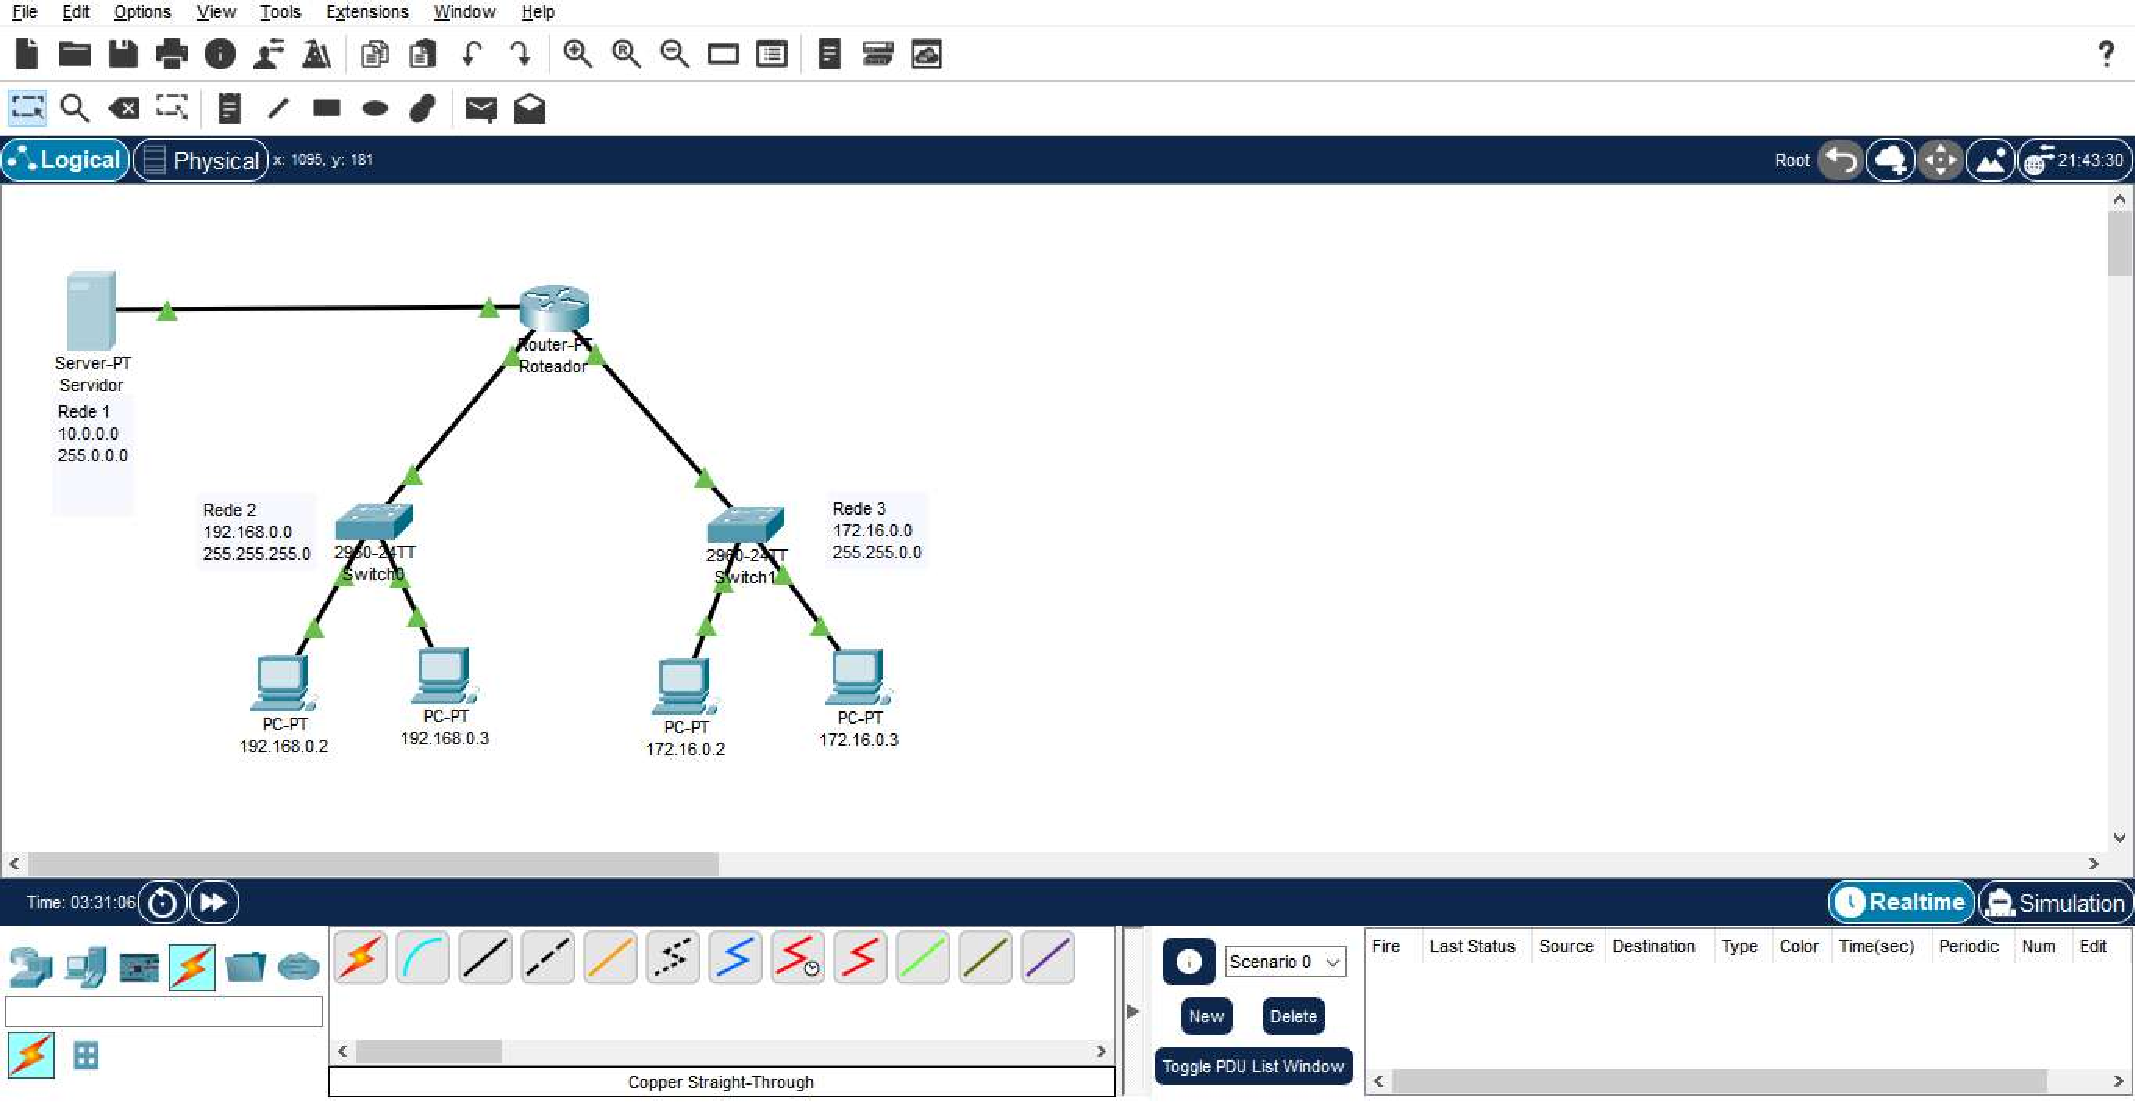
\includegraphics[width=.93\textwidth]{Figuras/firewallBase}
    \caption{Infraestrutura exemplo para a inclusão de \textit{firewall}.}\label{fig:firewallBase}
\end{figure}

\section{Configuração inicial do laboratório}\label{sec:configInicial}
Vamos detalhar as configurações atuais das redes. O servidor estará em uma rede local (LAN) composta apenas por ele mesmo. Note que o servidor possui com duas interfaces de rede, uma \textit{Gigabit Ethernet} e outra \textit{Fast Ethernet}. Nós utilizaremos apenas a \textit{Gigabit Ethernet}. O servidor terá o endereço IP \texttt{10.0.0.2} e estará na LAN \texttt{10.0.0.0}, com máscara \texttt{255.0.0.0}.  Chamaremos essa rede de \texttt{Rede 1} e o \textit{gateway} para essa rede será o \texttt{10.0.0.1}.

A \texttt{Rede 2} é composta por um \textit{switch} e dois PCs, tem endereço de rede \texttt{192.168.0.0} e máscara \texttt{255.255.255.0}. O primeiro PC tem o endereço IP \texttt{192.168.0.2} e o segundo PC tem o endereço IP \texttt{192.168.0.3}. Em ambos os casos, o \textit{gateway} será o \texttt{192.168.0.1}

Por sua vez, a \texttt{Rede 3} é composta por um \textit{switch} e dois PCs, tem endereço de rede \texttt{172.16.0.0} e máscara \texttt{255.255.0.0}. O primeiro PC tem o endereço IP \texttt{172.16.0.2} e o segundo PC tem o endereço IP \texttt{172.16.0.3}. Em ambos os casos, o \textit{gateway} será o \texttt{172.16.0.1}

Por fim, o roteador tem três interfaces \textit{Gigabit Ethernet} para se conectar ao servidor e as outras LANs. As interfaces têm as seguintes configurações:

\begin{itemize}
    \item A \texttt{GigabitEthernet0/0} tem endereço IP \texttt{10.0.0.1} e máscara \texttt{255.0.0.0}. Essa interface será ligada ao servidor.
    \item A \texttt{GigabitEthernet1/0} tem endereço IP \texttt{192.168.0.1} e máscara \texttt{255.255.255.0}. Essa interface será ligada ao \textit{switch} na \texttt{Rede 2}.
    \item A \texttt{GigabitEthernet2/0} tem endereço IP \texttt{172.16.0.1} e máscara \texttt{255.255.0.0}. Essa interface será ligada ao \textit{switch} na \texttt{Rede 3}.
\end{itemize}

Ainda no roteador, o roteamento escolhido foi o RIP e foram adicionadas as três redes \texttt{10.0.0.0}, \texttt{192.168.0.0} e \texttt{172.16.0.0}.

\section{Exercício}
Dada a configuração de rede atual, verifique se você consegue o seguinte:
\begin{itemize}
    \item Enviar um PDU de um PC na \texttt{Rede 1} para a \texttt{Rede 2}.
    \item Enviar um PDU de um PC na \texttt{Rede 1} para o servidor.
    \item Enviar um PDU do servidor para um PC na \texttt{Rede 2}.
\end{itemize}

Se não conseguiu, espere um pouco e tente novamente. É preciso algum tempo para as rotas estabilizarem.

\section{Configuração do \textit{Domain Name Service}}
Embora não seja necessário para a utilização do \textit{firewall}, para tornar o exemplo mais completo, vamos configurar um Sistema de Nomes de Domínio (\textit{Domain Name System} -- DNS) no próprio servidor. Basicamente um DNS é um sistema hierárquico e distribuído de gestão de nomes para  serviços ou qualquer máquina conectada à Internet ou a uma rede local. Em suma, o servidor DNS vai resolver um nome, isto é, traduzindo aquele nome em um endereço IP.

Para definir o DNS no servidor, basta seguir esses passos:
\begin{enumerate}[label*=\arabic*.]
\item Clique sobre o servidor, em seguida clique na aba \textit{Services}.
\item Na lateral esquerda, clique sobre a \textit{string}  \texttt{DNS}.
\item Na caixa de texto \textit{Name}, informe o nome do domínio que você vai definir. Nesse exemplo, colocamos o nome \semaspas{www.servidorft.com.br}.
\item Na caixa de texto \textit{Address}, defina o endereço IP daquele domínio que você vai definir. Nesse exemplo, colocamos o endereço \semaspas{10.0.0.2}. Note que é o endereço do próprio servidor, que também funcionará como servidor \textit{web}.
\item Depois de preenchidos o \textit{Name} e o \textit{Address}, clique no botão \keys{Add}.
\item Certifique-se que a configuração está salva, clicando no botão \keys{Save} e que o DNS está ativo selecionado a opção \textit{On} na parte superior.
\end{enumerate}

Agora, indique, em todos os PCs, o endereço do DNS está definido. Para isso, faça o seguinte em cada PC:

\begin{enumerate}[label*=\arabic*.]
\item Clique sobre o PC.
\item Selecione a aba \textit{Config}.
\item Informe o endereço IP \semaspas{10.0.0.2} na caixa de texto \textit{DNS Server}.
\end{enumerate}

\section{Exercício}
Escolha um PC na sua rede e verifique se o servidor \textit{Web} está ativo. Para isso, faça o seguinte:

\begin{enumerate}[label*=\arabic*.]
\item Clique sobre o PC.
\item Selecione a aba \textit{Desktop} e em seguida selecione o \textit{Web Browser}.
\item Na caixa de texto \textit{URL}, informe o nome do servidor \semaspas{www.servidorft.com.br}.
\end{enumerate}

Se deu certo, deve aparecer uma página com o título \textit{Cisco Packet Tracer}. Repita esse procedimento em todos os PCs, para se certificar que funciona para todos.

\section{Funcionamento básico do \textit{firewall}}\label{sec:funcBasicoFirewall}

Cada serviço disponível na rede está vinculado a uma porta específica. Por exemplo, o serviço \textit{web} que usa o  Protocolo de Transferência de Hipertexto (\textit{Hypertext Transfer Protocol} -- HTTP) usa a porta 80; o serviço FTP, usa a porta 21; e o serviço DNS usa a porta 53. Esses serviços também utilizam protocolos específicos na camada de transporte. Esses protocolos podem ser o Protocolo de Controle de Transmissão (\textit{Transmission Control Protocol} -- TCP) ou o Protocolo de Datagrama do Usuário (\textit{User Datagram Protocol} -- UDP).

Um \textit{firewall} permite ou nega acessos observando os protocolos utilizados, os endereços IP de origem e destino das conexões, e também as portas de origem e destino dos pacotes. Assim, as regras de segurança são estabelecidas com base nesses parâmetros.

\section{Configuração do \textit{firewall}}\label{sec:configFirewall}
Agora, faremos a configuração do \textit{firewall} no servidor. Para esse exemplo, vamos permitir (\textit{Allow}) o acesso dos PCs aos serviços DNS e \textit{Web}. Mais a frente, no exercício, terminaremos a configuração para negar (\textit{Deny}) o acesso dos PCs aos serviços ICMP e de transferência de arquivos (com o \textit{file transfer protocol} -- FTP). Lembrando que a negação do serviço ICMP vai evitar a conexão pelo comando \Comando{ping}.

Para configurar o \textit{firewall}, vamos executar os seguintes passos:

\begin{enumerate}[label*=\arabic*.]
\item Clique sobre o servidor e em seguida, clique na aba \textit{Desktop}.
\item Clique sobre o ícone do \textit{firewall IPv4}. Cuidado, pois também há o \textit{firewall IPv6} que não utilizaremos neste exemplo.
\item Na seção \textit{Service}, selecione a opção \textit{On} para deixar esse serviço ativo.
\item Na seção \textit{Interface}, selecione a opção \textit{GigabitEthernet1}, que é a interface a qual o \textit{firewall} vai observar.
\item Para permitir o serviço DNS faça o seguinte:  
   \begin{enumerate}[label*=\arabic*.]
      \item Na caixa de opções \textit{Action}, selecione \textit{Allow}.
      \item Na caixa de opções \textit{Protocol}, selecione \textit{UDP}.
      \item Na caixa de texto \textit{Remote IP}, preencha com o endereço IP da rede da qual virão os pacotes (nesse exemplo, a rede \texttt{192.168.0.0}).
      \item Na caixa de texto \textit{Remote Wildcard Mask}, preencha com a máscara invertida da rede da qual virão os pacotes (nesse exemplo, a máscara da rede é \texttt{255.255.255.0} e a máscara invertida -- que você deverá preencher -- é a \texttt{0.0.0.255}).
      \item Na caixa de texto \textit{Remote port}, preencha com a \textit{string} \texttt{any}. Essa \textit{string} informa que a porta de origem da conexão pode ser qualquer uma.
      \item Na caixa de texto \textit{Local port}, informe a porta 53 (a porta do serviço DNS).
      \item Depois que as informações forem preenchidas, clique em \keys{Add}.
   \end{enumerate}
\item Para permitir o serviço \textit{Web} repita o procedimento do item 5, substituindo o seguinte:
   \begin{enumerate}[label*=\arabic*.]
      \item Substituir o protocolo (no item 5.2) por \textit{TCP}.
      \item Substituir a \textit{Local port} (no item 5.6), pela porta 80 (a porta do serviço \textit{web}).
    \end{enumerate}
\end{enumerate}

A negação dos serviços ocorre de forma similar à liberação. A diferença é que, na caixa de opções \textit{Action}, você deve selecionar a opção \textit{Deny}. 

\section{Exercício}
Na \Cref{sec:configFirewall}, fizemos a configuração do \textit{firewall} para permitir dois serviços (DNS e \textit{web}) para a \texttt{Rede 2} (\texttt{192.168.0.0}). Nesse exercício, termine a configuração para bloquear o protocolo ICMP e o FTP na Rede 2 e faça a configuração completa para a \texttt{Rede 3} (\texttt{172.16.0.0}). Lembrando que o serviço FTP utiliza o protocolo TCP na camada de transporte e atua na porta 21. O serviço ICMP também utiliza o protocolo TCP na camada de transporte e atua na porta 23.

Ao final, a configuração do \textit{firewall} deve ficar conforme a \Cref{fig:configFirewall}. Depois que a configuração do \textit{firewall} estiver completa, faça testes para verificar se os serviços estão realmente bloqueados e liberados. 

\begin{figure}[!htb]
    \centering
    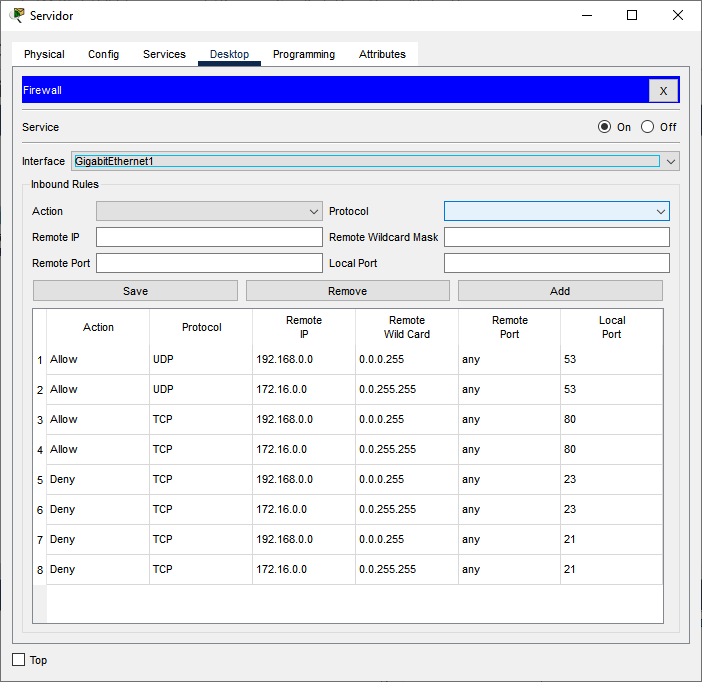
\includegraphics[width=.9\textwidth]{Figuras/configFirewall}
    \caption{Configuração final do \textit{firewall} no exemplo.}\label{fig:configFirewall}
\end{figure}

\chapter*{Epílogo}\label{chp:epilogo}
\addcontentsline{toc}{chapter}{Epílogo}

Este texto foi concebido para apoiar as aulas práticas da disciplina Redes de Comunicação I. Nem sempre é possível a utilização de equipamentos físicos em quantidade suficiente para os estudantes. Por isso, a utilização de um ambiente simulado, próximo do real, ajuda os estudantes a colocar em prática os conhecimentos adquiridos na disciplina.

Temos consciência que este texto não está completo. Portanto, as novas versões devem trazer mais conteúdo, além de corrigir eventuais erros da versão atual.  É importante destacar que o \CPT possui muitos recursos que não foram explorados aqui. Porém, a expectativa é que o conteúdo abordado nesse texto seja apenas o ponto de partida para outras práticas mais interessantes, que explorem situações mais particulares, e prepare os estudantes para os desafios no mundo real. 

Por fim, o leitor desse texto pode ficar à vontade para sugerir novas práticas ou novos conteúdos a serem abordados nas próximas versões desse texto. As críticas, sugestões e elogios podem ser feitas pelo e-mail a seguir ou nas redes sociais.

Bom proveito!

\href{mailto://gradvohl@ft.unicamp.br}{\faIcon{at}\xspace gradvohl@ft.unicamp.br}

\href{https://github.com/gradvohl}{\faIcon{github}/gradvohl}

\href{https://orcid.org/0000-0002-6520-9740}{\textcolor{orcidlogocol}{\faIcon{orcid}}/0000-0002-6520-9740}

\href{https://www.linkedin.com/in/andregradvohl}{\textcolor{linkedinlogocol}{\faIcon{linkedin}}/andregradvohl}

\href{https://twitter.com/AGradvohl}{\textcolor{twitterlogocol}{\faIcon{twitter}}/AGradvohl}

\href{https://fosstodon.org/@gradvohl}{\textcolor{mastodonlogocol}{\faIcon{mastodon}} @gradvohl@fosstodon.org}

\vspace*{\fill}
\begin{flushright}
    \textit{The greatest teacher, failure is.}\\
    Yoda.
\end{flushright}


%%%% Licença
\chapter*{Licença de uso}\label{chp:licenca}
\addcontentsline{toc}{chapter}{Licença de uso}

\doclicenseThis

Essa licença permite que o usuário copie e redistribua o material em qualquer meio ou formato. Permite ainda que o usuário remixe, transforme, e use o material para complementar outros materiais para qualquer propósito, mesmo os comerciais.

 Detalhes sobre a licença estão disponíveis no \textit{site} a seguir:
 \begin{center}
    \url{https://creativecommons.org/licenses/by/4.0}     
 \end{center}

Todos os arquivos usados nas tarefas e o código fonte em \LaTeX{} deste texto estão disponíveis no site do GitHub conforme o endereço a seguir. Esse texto está armazenado indexado no site do Zenodo indicado no DOI a seguir.

\faGithub\ GitHub: \url{https://github.com/gradvohl/LabRedesComputadores}

\def\myDOI{10.5281/zenodo.7534173}
DOI: \url{https://doi.org/\myDOI}%10.5281/zenodo.7534173}

Para citar este texto, use as seguintes informações:

\noindent
{\sc Gradvohl, A. L. S.} Laboratório de Redes de Computadores com Cisco Packet Tracer. Zenodo. DOI: \href{http://doi.org/\myDOI}{10.5281/zenodo.7534173}, 2023.

\end{document}
